\chapter{PHYSICS OBJECT RECONSTRUCTION} \label{reco}

In the early days of particle physics experimentation, charged particles were visually identified by analyzing photographs of the ionization tracks left behind in cloud chambers and bubble chambers. Given the higher collision energies and instantaneous luminosities demanded by modern experiments, the amount of information recorded for a collision event renders such visual analyses intractable. The final state particles produced by a proton collision at the LHC are recorded as electronic signals by the CMS detector, and the accurate interpretation of these signals as physics objects is what enables the full reconstruction of the collision's aftermath. The definition and reconstruction of the standard physics objects, with an emphasis on those used by the \VHbb\ analysis, are described in this chapter.

\section{Particle Flow Algorithm}

The hermetic design of the CMS detector and the granularity of its subsystems enabled the first successful deployment of a \textit{particle flow (PF)} based reconstruction algorithm at a hadron collider experiment.\cite{PARTICLEFLOW} Although the individual subsystems are capable of reconstructing the particles for which they were designed, a more accurate and global event description can be achieved by combining the measurements obtained by the subsystems as a whole. Since its commissioning, the PF algorithm has been used online to improve the efficiency of the High-Level Trigger (HLT) and offline to improve the quality of the reconstructed particle candidates considered by physics analyses.

The PF algorithm starts by collecting the detector-level objects, or \textit{elements}, produced by each detector subsystem: the silicon tracker and muon chambers both provide charged particle \textit{tracks}, while the electromagnetic calorimeter (ECAL) and hadronic calorimeter (HCAL) both provide \textit{clusters} of absorbed energy. A \textit{link algorithm} which tests the compatibility of pairs of elements from different subsystems is used to generate \textit{blocks} of elements that are directly linked or indirectly linked through common elements. Individual particles are subsequently identified and reconstructed within each block, starting with muons then proceeding to electrons, photons, and charged and neutral hadrons. As particles are reconstructed, the elements associated with that particle are removed from the block such that each particle is reconstructed from a set of unique elements. Once all the blocks have been processed and all particles in the event have been identified and reconstructed, a post-processing algorithm is used to correct misidentified or misreconstructed muons with large transverse momentum \pT which can artificially increase the reconstructed missing transverse momentum \pTmiss\ in the event.

\begin{figure}[htbp]
  \centering
    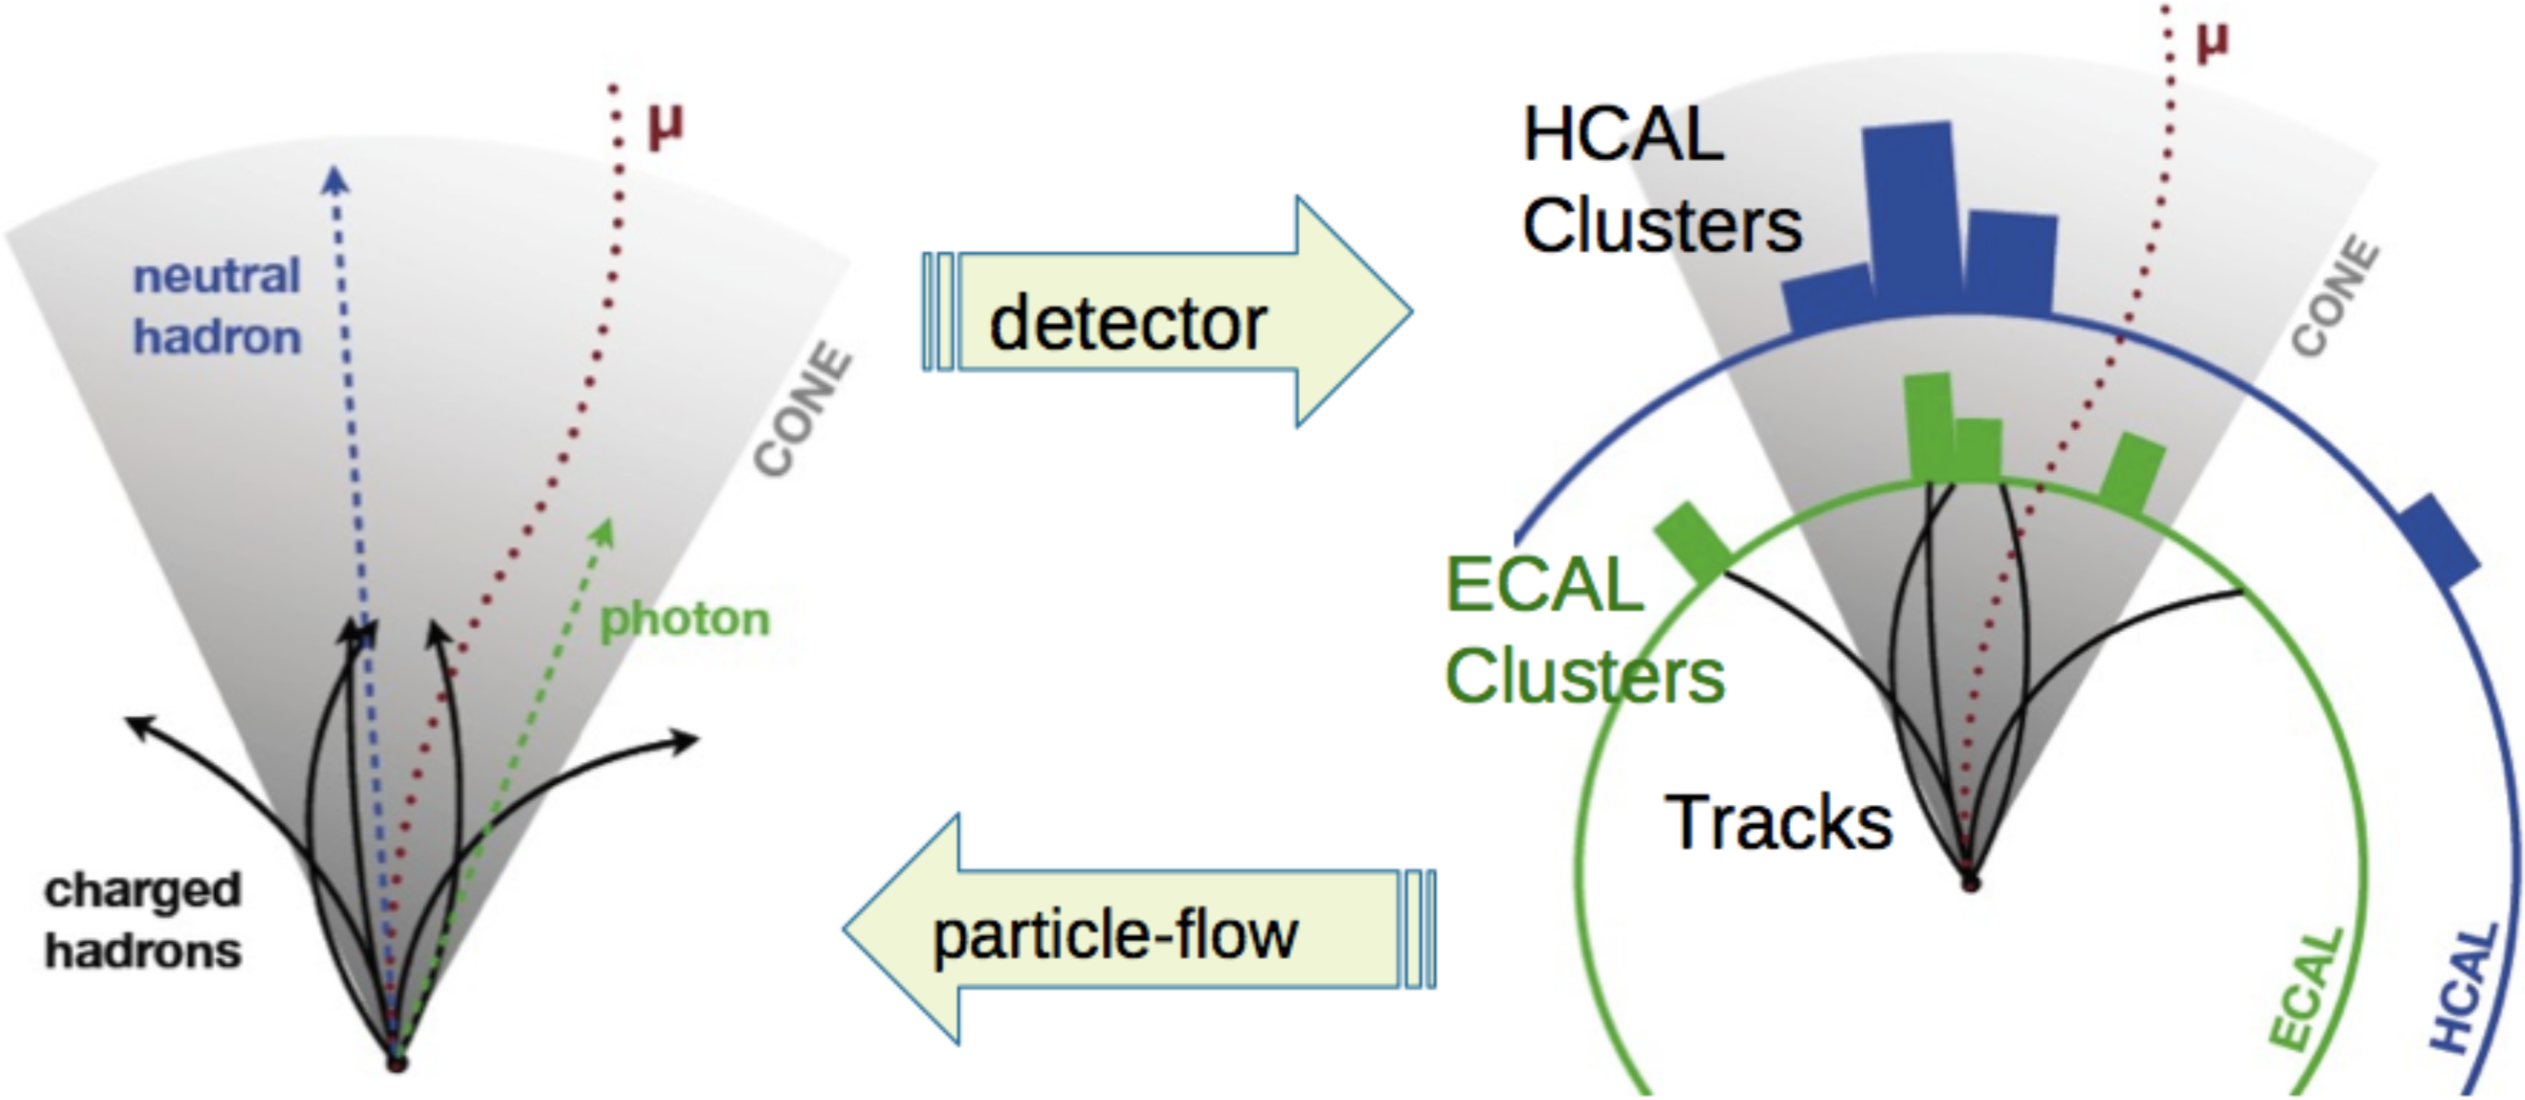
\includegraphics[width=5in]{images/pfdiagram}
    \caption[Particle Flow Infographic]{An infographic illustrating the particle flow reconstruction paradigm.\cite{pfdiagram}}
    \label{fig:pfdiagram}
\end{figure}

At this stage, the particle candidates proposed by the PF algorithm are ready to be used in physics analyses. In practice, the particle candidates are processed further by passing them to algorithms which employ different clustering strategies to reconstruct jets. Finally, The candidate particles and jets which satisfy the additional criteria recommended by the various physics object groups (POGs) within the CMS collaboration become the standard physics objects considered by the physics analyses.

\subsection{Detector-level Objects}

Each detector subsystem produces objects which become the fundamental inputs to the PF algorithm. The two main types of detector-level objects are charged particle tracks, with a distinction between tracks from the silicon tracker and standalone muon tracks from the muon chambers, and calorimeter clusters. By considering these objects together, the full information gathered by the detector may be brought to bear for the task of identifying and reconstructing particles.

\subsubsection{Tracks}

The silicon tracker, the inner-most detector subsystem of the CMS detector, reconstructs tracks from \textit{hits}, which are clusters of signals gathered by the pixel and strip trackers. This task quickly becomes a combinatorial challenge because of its dense operating environment due to \textit{pileup}. The bunched nature of the LHC's proton beams results in multiple proton-proton collisions each time they cross the interaction point as illustrated in Figure \ref{fig:pileup}, and those collisions which overlap the one of interest are deemed pileup interactions. Although the number of hits in the tracker increases linearly with pileup, the number of possible combinations of hits to form tracks grows exponentially.

\begin{figure}[htbp]
  \centering
    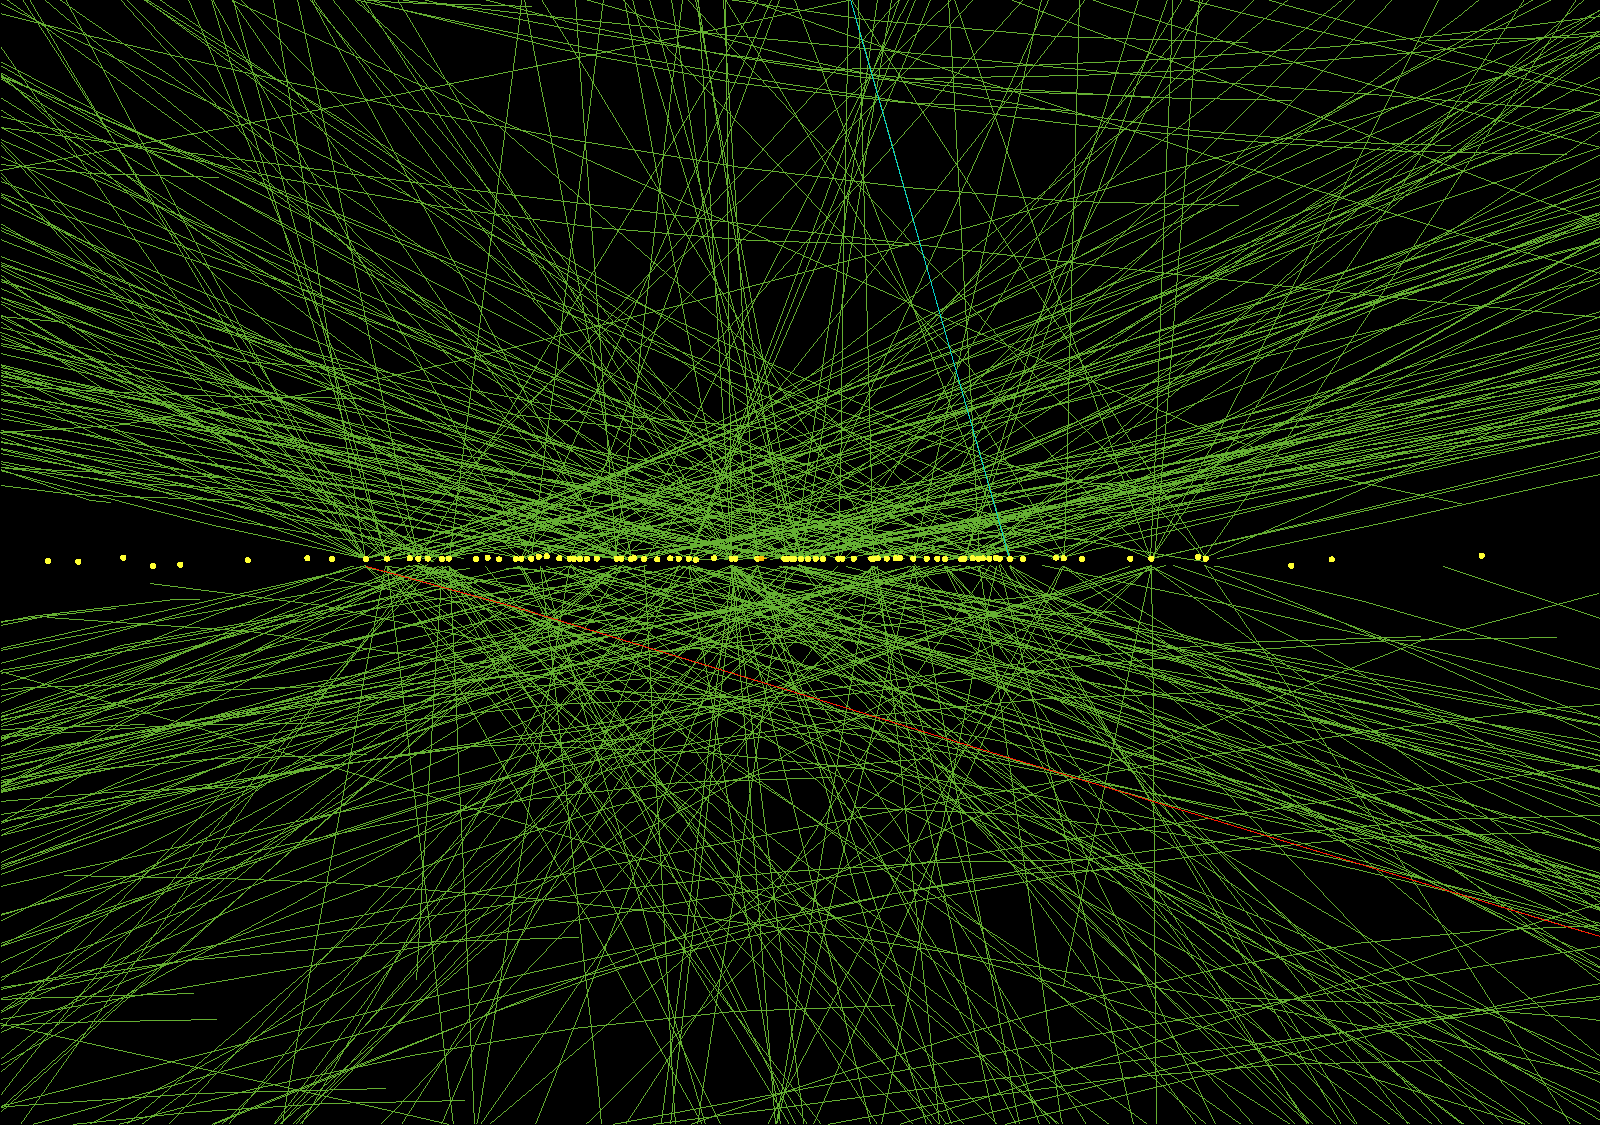
\includegraphics[width=4in]{images/pileup}
    \caption[Event Display of High-Pileup Collision Event]{An event display for a collision from the high-pileup run 198609 which shows 78 reconstructed vertices and their associated charged particle tracks.\cite{pileup}}
    \label{fig:pileup}
\end{figure}

In order to accurately and quickly reconstruct tracks, an iterative tracking algorithm\cite{ITERTRACK} is employed by the CMS experiment which applies several iterations of a combinatorial track finder (CTF) based on Kalman filtering\cite{CMSTRACKRECO} to a collection of hits. Each iteration of the CTF proceeds through the following stages:

\begin{itemize}
  \item \textbf{Seed Generation:} Initial trajectory candidates composed of three hits or two hits and a beamspot or vertex constraint are proposed as seeds.
  \item \textbf{Trajectory Building:} The seeds are extrapolated towards compatible hits in subsequent layers and also towards a single ``invalid'' or fake hit to account for the case where the corresponding hit was not recorded. A Kalman filter then updates the trajectory based on the compatible hit to form track candidates. This extrapolation procedure terminates upon reaching the outermost layer of the tracker or a when ``stop condition'' is satisfied, such as surpassing a maximum number of invalid hits. Because a single seed may produce multiple track candidates and different seeds may produce the same track candidate, an ambiguity resolution based on the fraction of hits shared between pairs of track candidates is applied to prevent double counting.
  \item \textbf{Track Fitting:} The collection of hits for each track candidate is refitted by a Kalman filter and smoother to obtain optimal estimates of the track parameters illustrated in Figure \ref{fig:track_params}: the signed transverse curvature $q\pT$, the polar angle $\cot \theta_{0}$, the azimuthal angle $\phi_{0}$, the longitudinal impact parameter $d_{z}$, and the signed transverse impact parameter $d_{0}$, all of which are defined at the point of closest approach to the beam axis.
\end{itemize}

\begin{figure}[htbp]
  \centering
    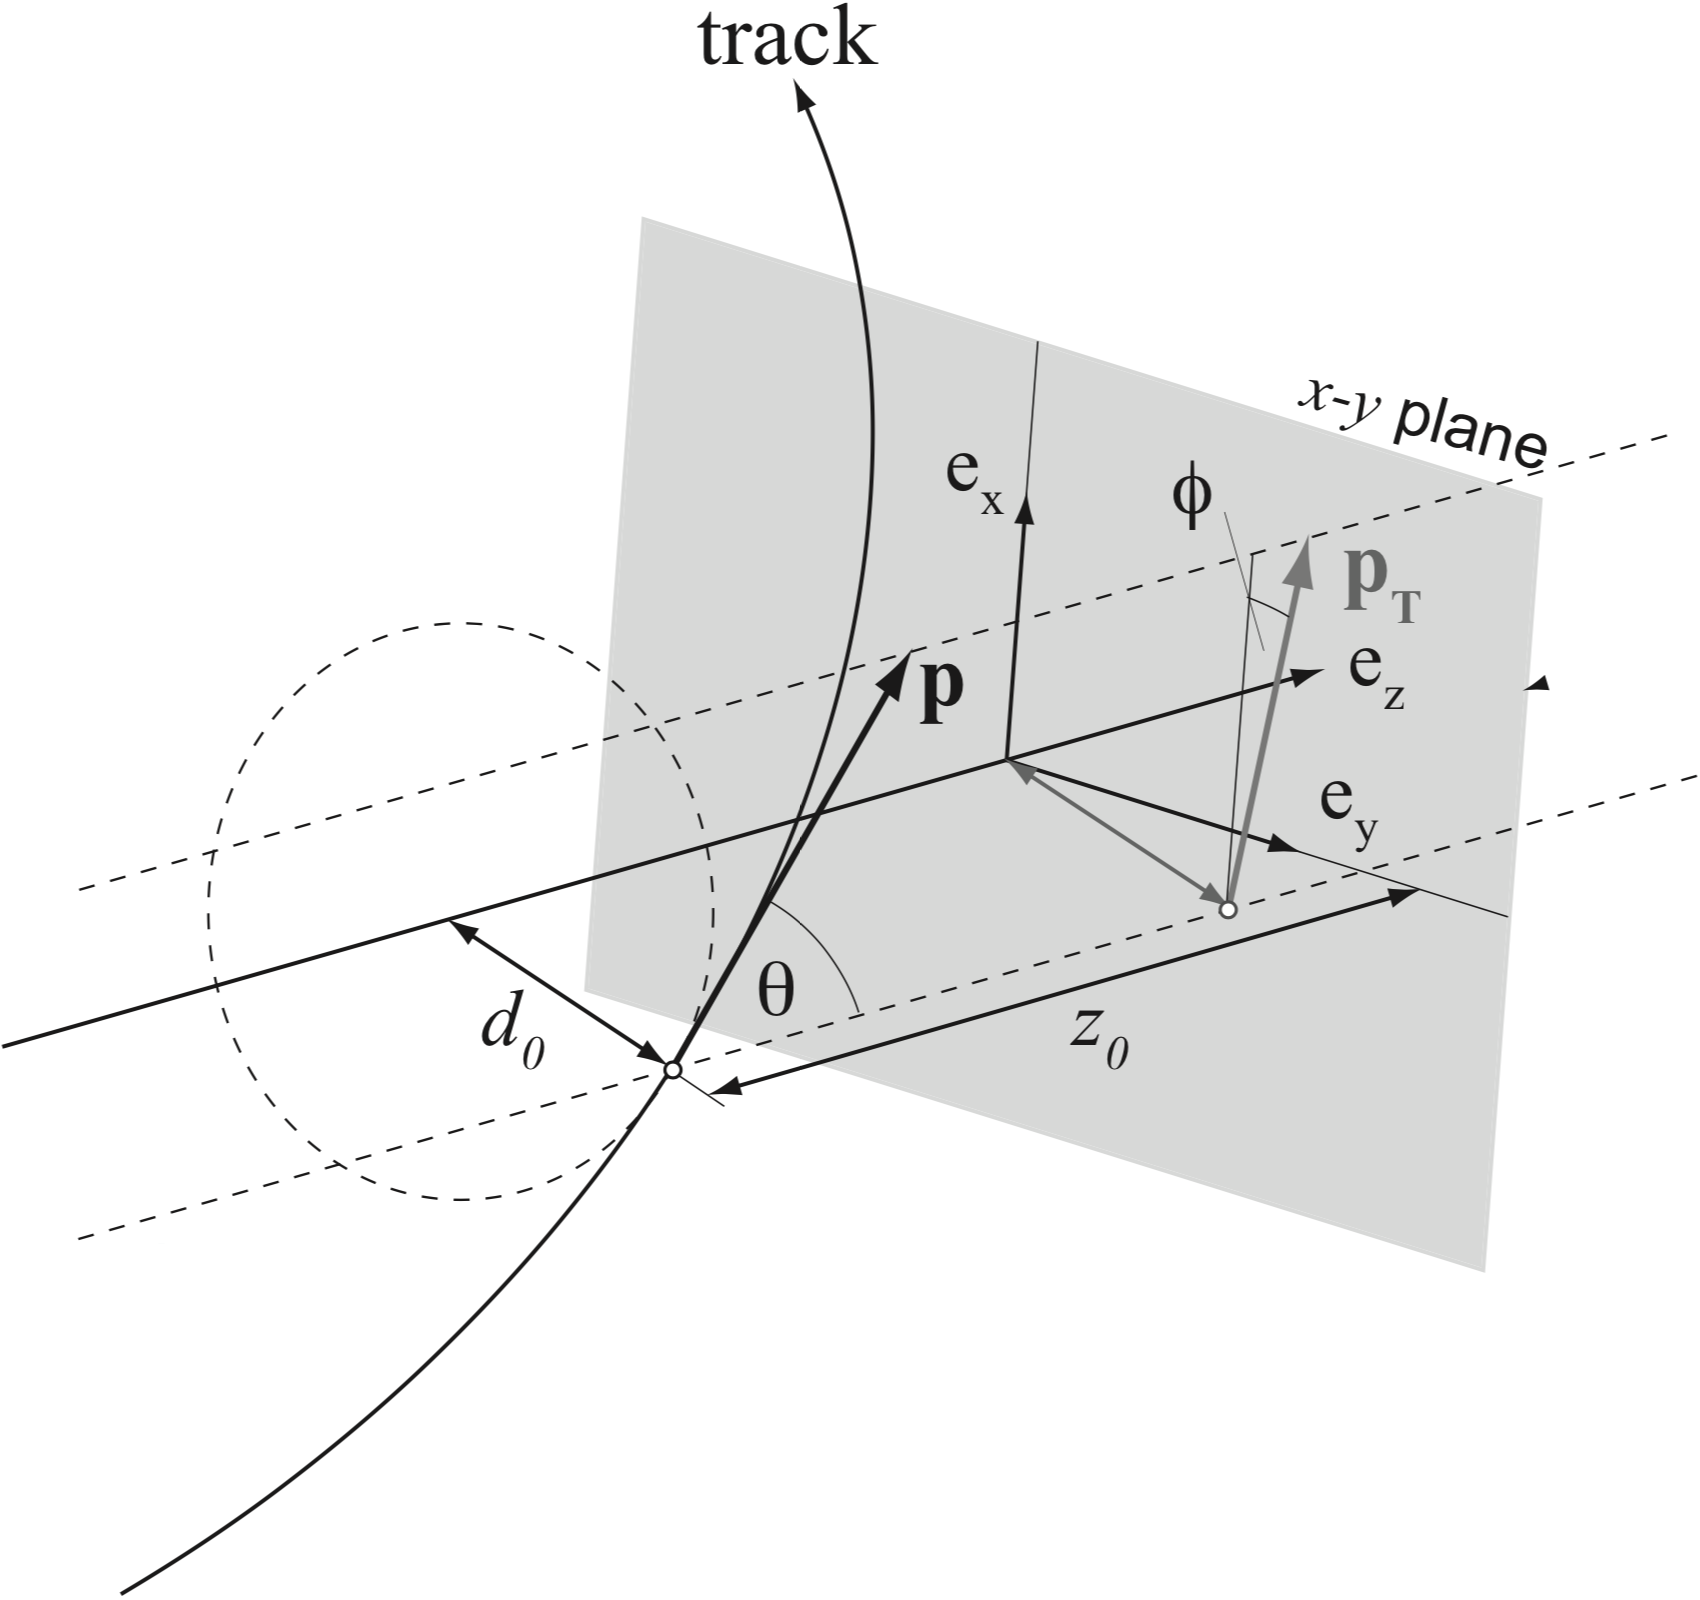
\includegraphics[width=3.5in]{images/track_parameters}
    \caption[Charged Particle Trajectory Parameterization]{The parameterization of a charged particle's trajectory through a magnetic field.\cite{salzburger}}
    \label{fig:track_params}
\end{figure}

The CTF is run for a total of ten iterations. The first iteration seeks to reconstruct the easiest tracks which originate close to the interaction point, also called \textit{prompt} tracks, and have high \pT. The last two iterations attempt to reconstruct muons and involves muon tracks which are described in further detail in section \ref{standalonemuontrack}. Because successive iterations face increasingly difficult tasks, the hits associated with selected track candidates are masked in subsequent iterations to reduce the combinatorial complexity. The seeds and reconstruction targets of the ten iterations are summarized by Table \ref{tbl:itertrack}.

\begin{table}[htbp]
  \caption[Iterative Tracking Summary]{A summary of the ten tracking iterations used by the CMS tracker. The variable $R$ in the final column denotes the distance from the beam axis to the production position of the targeted track.\cite{PARTICLEFLOW}}
  \label{tbl:itertrack}
  \small
  \begin{tabularx}{6.5in}{XXl}
    \hline
    Iteration & Seed Type            & Reconstructed Tracks                    \\
    \hline
    1         & pixel triplets       & prompt, high \pT                        \\
    2         & pixel triplets       & from b hadron decays, $R \lesssim 5$ cm \\
    3         & pixel triplets       & prompt, low \pT                         \\
    4         & pixel pairs          & recover high \pT                        \\
    5         & pixel+strip triplets & displaced, $R \lesssim 7$ cm            \\
    6         & strip triplets/pairs & very displaced, $R \lesssim 25$ cm      \\
    7         & strip triplets/pairs & very displaced, $R \lesssim 60$ cm      \\
    8         & pixel+strip pairs    & inside high \pT jets                    \\
    9         & muon-tagged tracks   & muons                                   \\
    10        & muon detectors       & muons                                   \\
    \hline
  \end{tabularx}
\end{table}

\begin{figure}[htbp]
  \centering
  \mbox{
    \subfigure [] {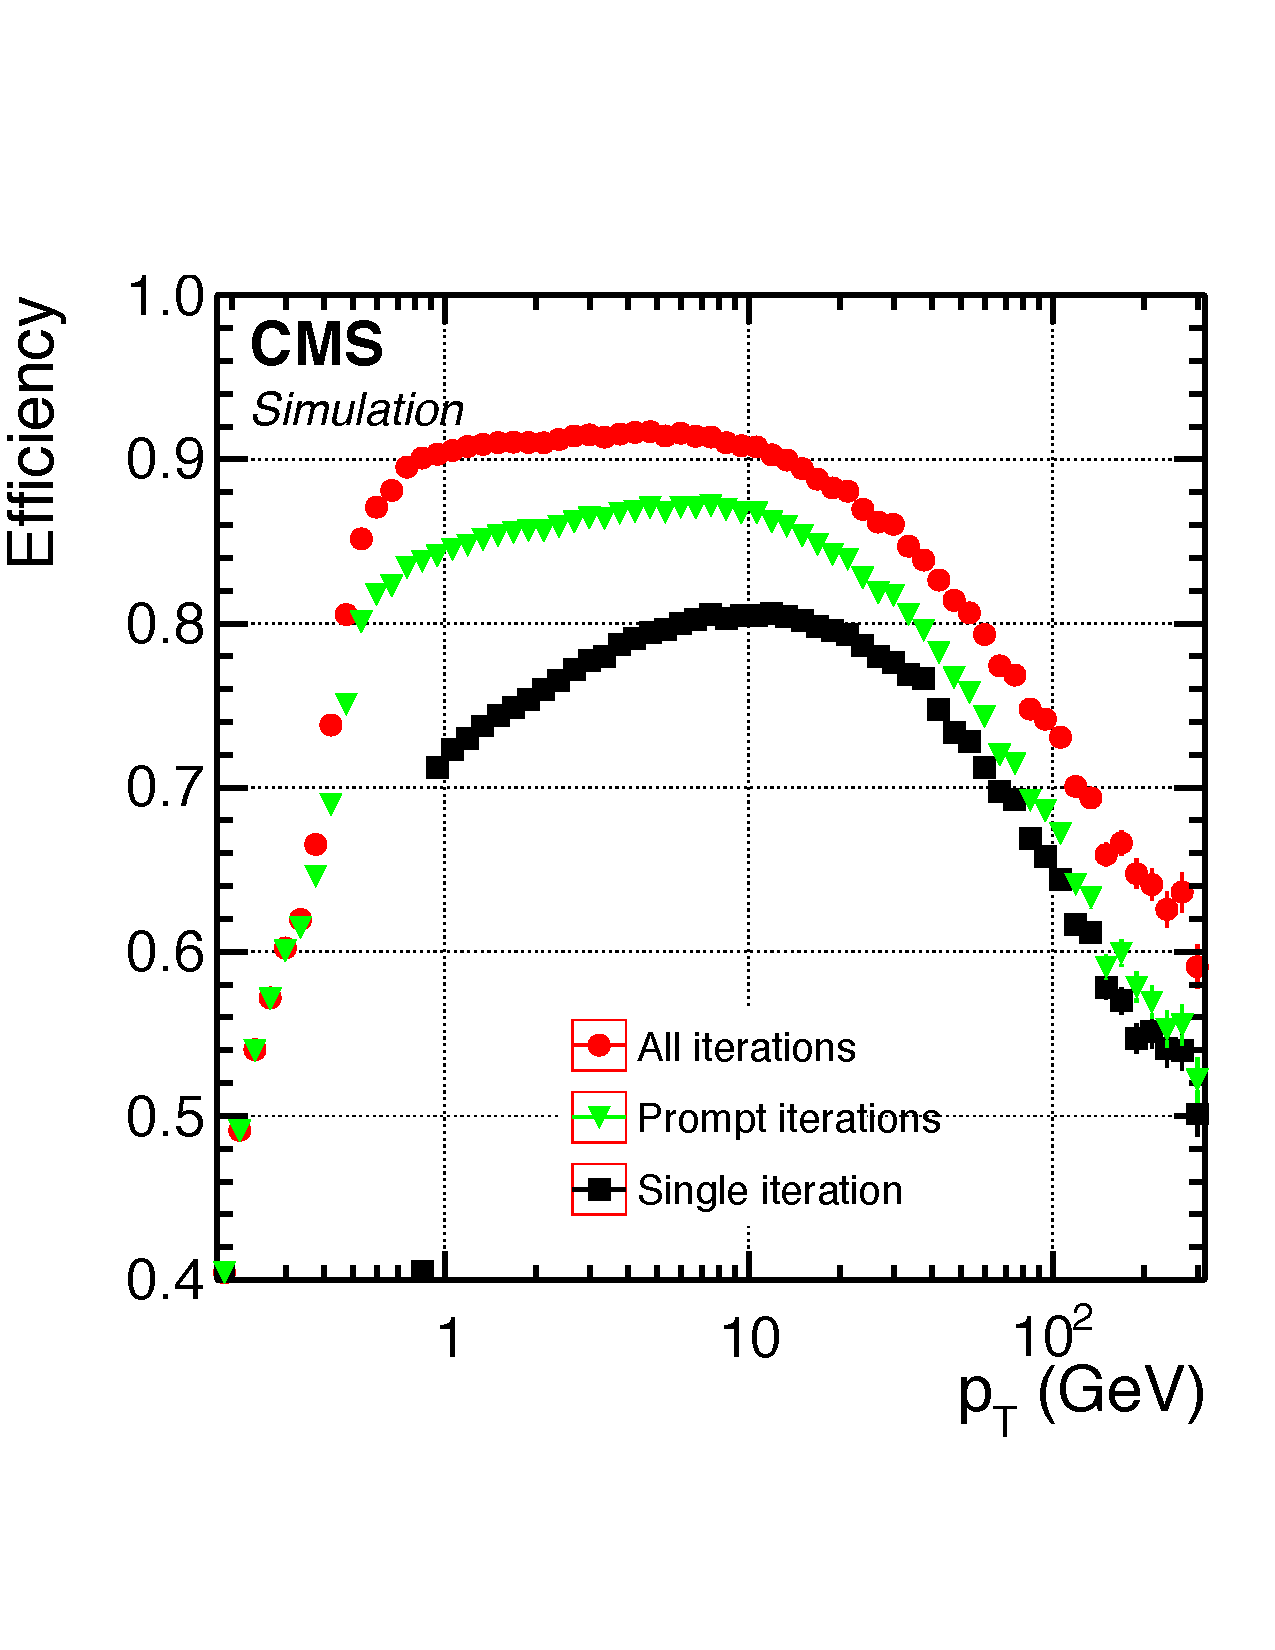
\includegraphics[scale=0.35]{images/pftrack_eff}} \qquad
    \subfigure [] {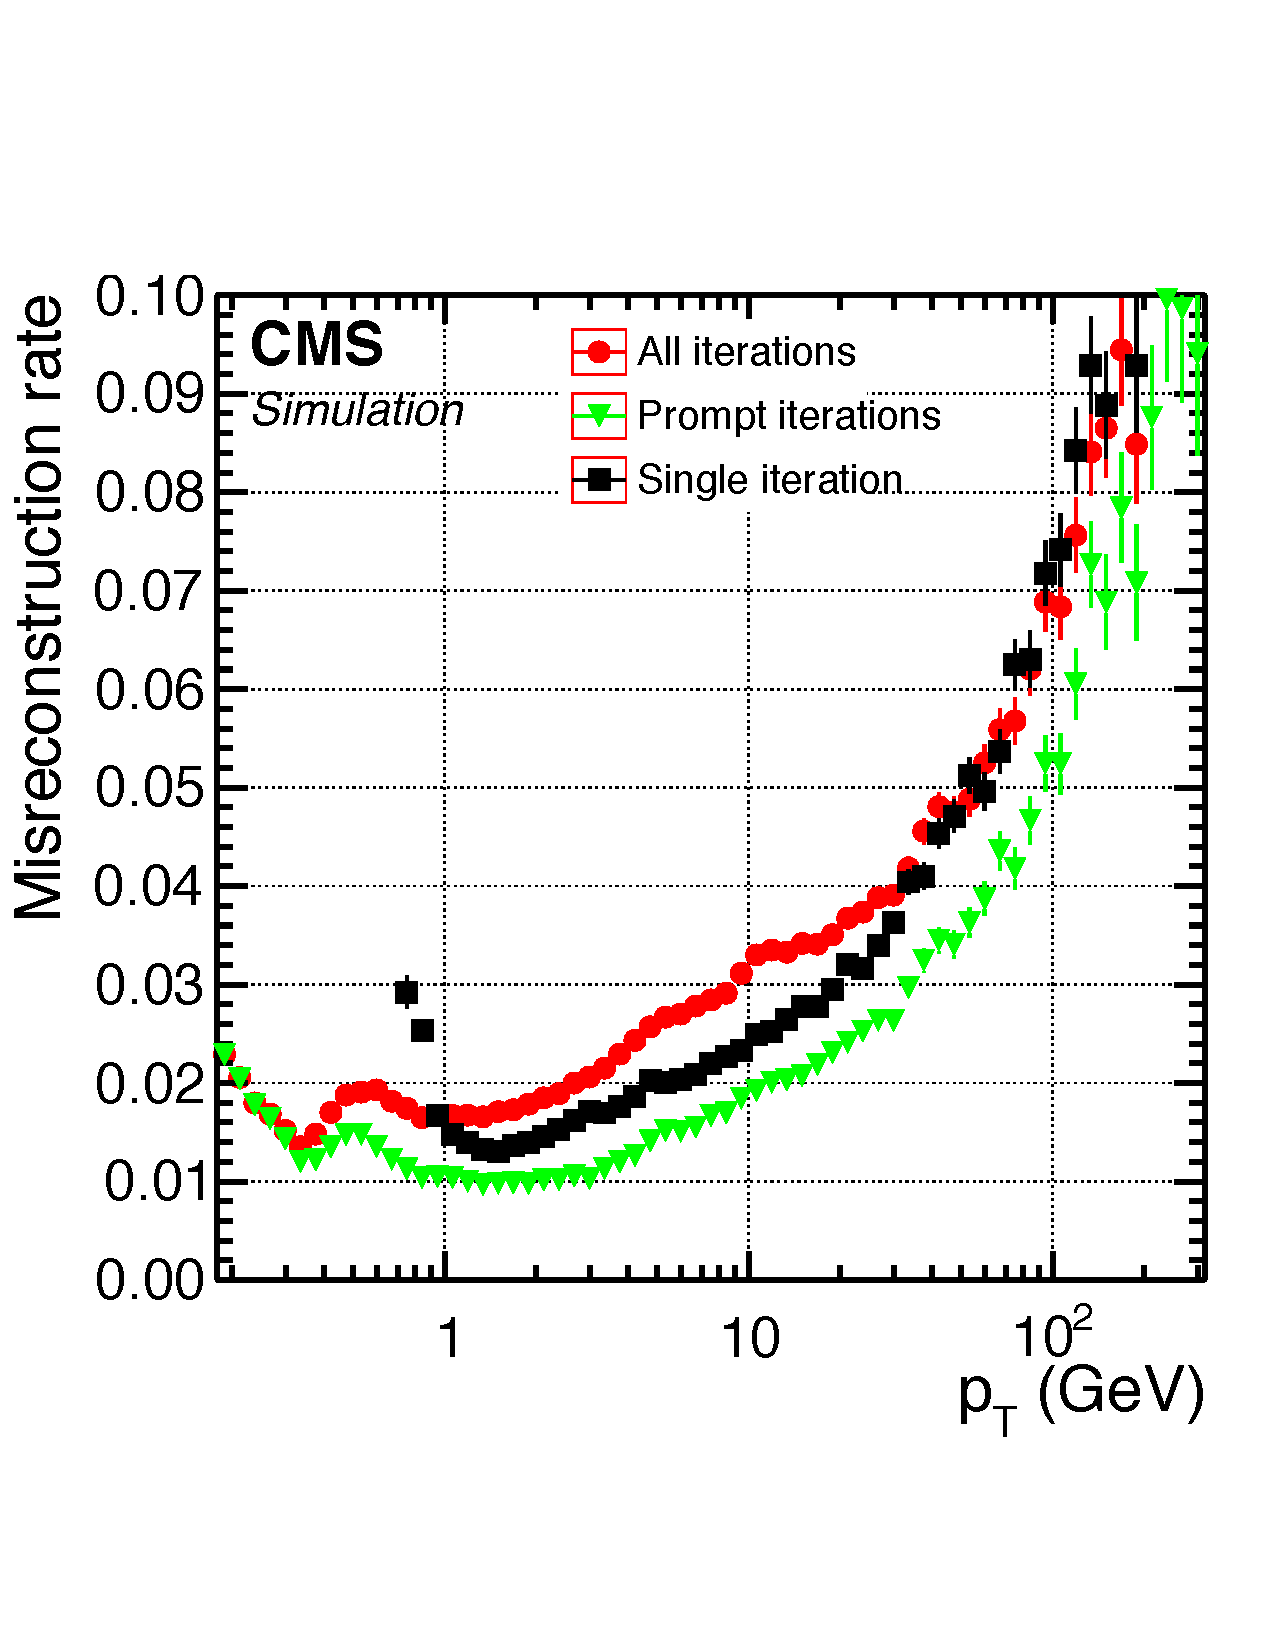
\includegraphics[scale=0.35]{images/pftrack_misreco}} \qquad
  }
  \caption[Track Reconstruction Performance]{The A) tracking efficiency and B) misreconstruction rate of charged hadron tracks in simulated multijet events for a single, global iteration of the combinatorial track finder (black squares), the prompt iterations (iterations 1, 2, 3, 4, 5, and 7) of the iterative tracking method (green triangles), and the full iterative tracking method (red circles) as a function of track \pT.\cite{PARTICLEFLOW}}
    \label{fig:pftrack_perf}
\end{figure}

The tracking efficiency and misreconstruction rate are shown in Figure \ref{fig:pftrack_perf}. The full iterative tracking method achieves a 90\% reconstruction efficiency for tracks with \pT\ between 1 \GeV\ and 10 \GeV, to be compared with the 70-80\% efficiency of the global CTF, and maintains an approximately 8-10\% higher efficiency than the global CTF for tracks with $\pT > 100 \GeV$. Although the iterative tracking method incurs a slightly higher misreconstruction rate than the global CTF, it is able to reconstruct over half of the tracks missed by the global CTF while running twice as fast.

\subsubsection{Calorimeter clusters}

The ECAL and HCAL, which are the intermediate detector subsystems of the CMS detector, reconstruct energy clusters left behind by traversing particles. The electromagnetic interactions of particles with the ECAL materials induce electromagnetic showers which deposit their energy in lead tungstate crystals. The strong interactions of particles with the HCAL materials induce hadronic showers and jets which deposit their energies in alternating layers of brass or steel absorbing plates and plastic scintillator. The electronic signals produced by these showers are measured by the cells of their respective calorimeter.

The ECAL clusters are seeded by cells which contain a local energy maxima above a detector-dependent threshold. The \textit{Island algorithm} is used in both the ECAL barrel and endcaps to cluster the eight cells directly adjacent to the seed in the $\eta\phi$-plane with measured energies above twice the noise level, while the \textit{hybrid algorithm} is used in the ECAL barrel only and forms bars that are 3 or 5 crystals wide in $eta$ before searching along the $phi$-direction. Both of these algorithms propose \textit{topological clusters} which are themselves clustered into \textit{superclusters}. The most energetic topological cluster is used as the supercluster seed, and nearby clusters are gathered into a supercluster with some spread in the $phi$-direction to recover the energy from photon conversions and bremsstrahlung which are spread by the solenoid's magnetic field. Although 94\% of the energy of a photon or electron is contained by a $3\times3$ cluster of crystals, and up to 97\% for $5\times5$ clusters, detector materials before the ECAL result in energy losses which are accounted for by applying corrections to the supercluster energies. Clusters are similarly constructed using information from the HCAL, although the algorithms proceed by considering only those four cells which share an edge with the seed cell. A visualization of ECAL and HCAL clusters are shown in Figure \ref{fig:caloclusters}.

\begin{figure}[htbp]
  \centering
  \mbox{
    \subfigure [] {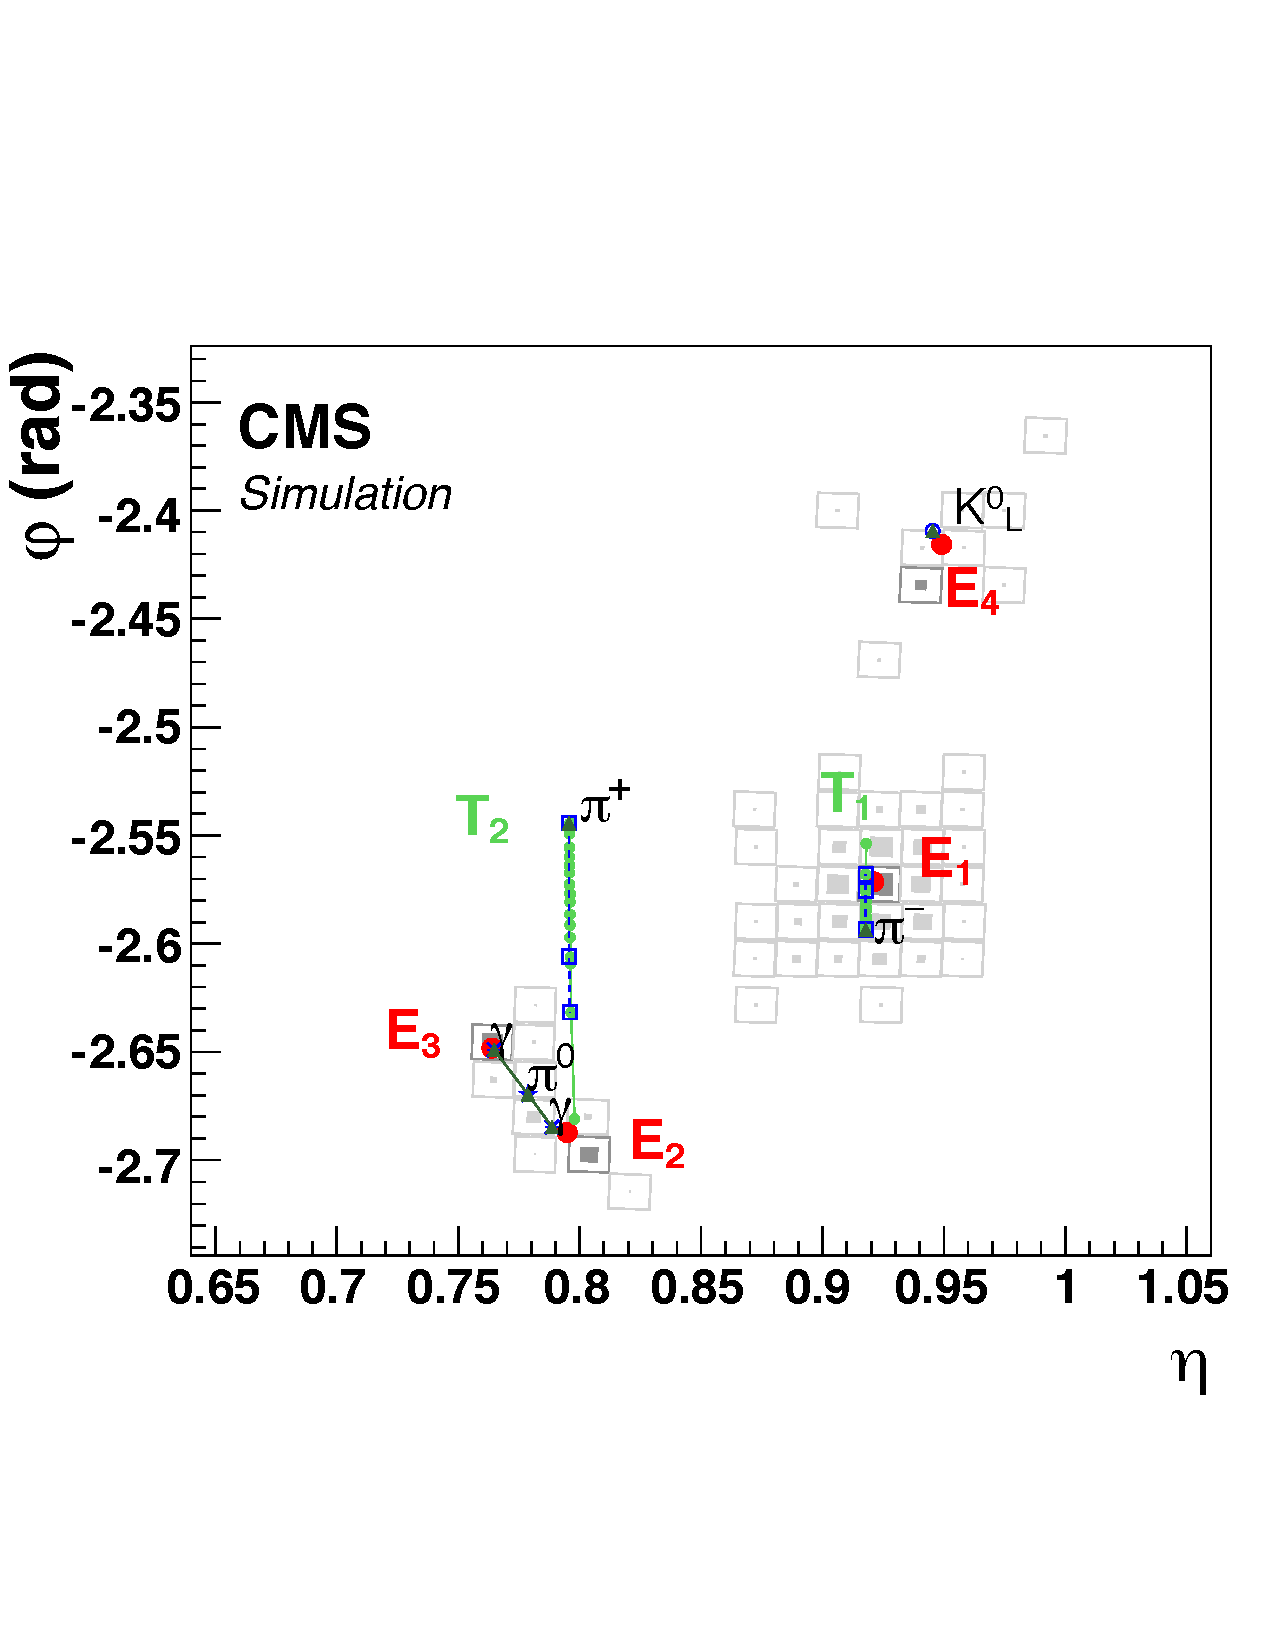
\includegraphics[scale=0.35]{images/ecalclusters}} \qquad
    \subfigure [] {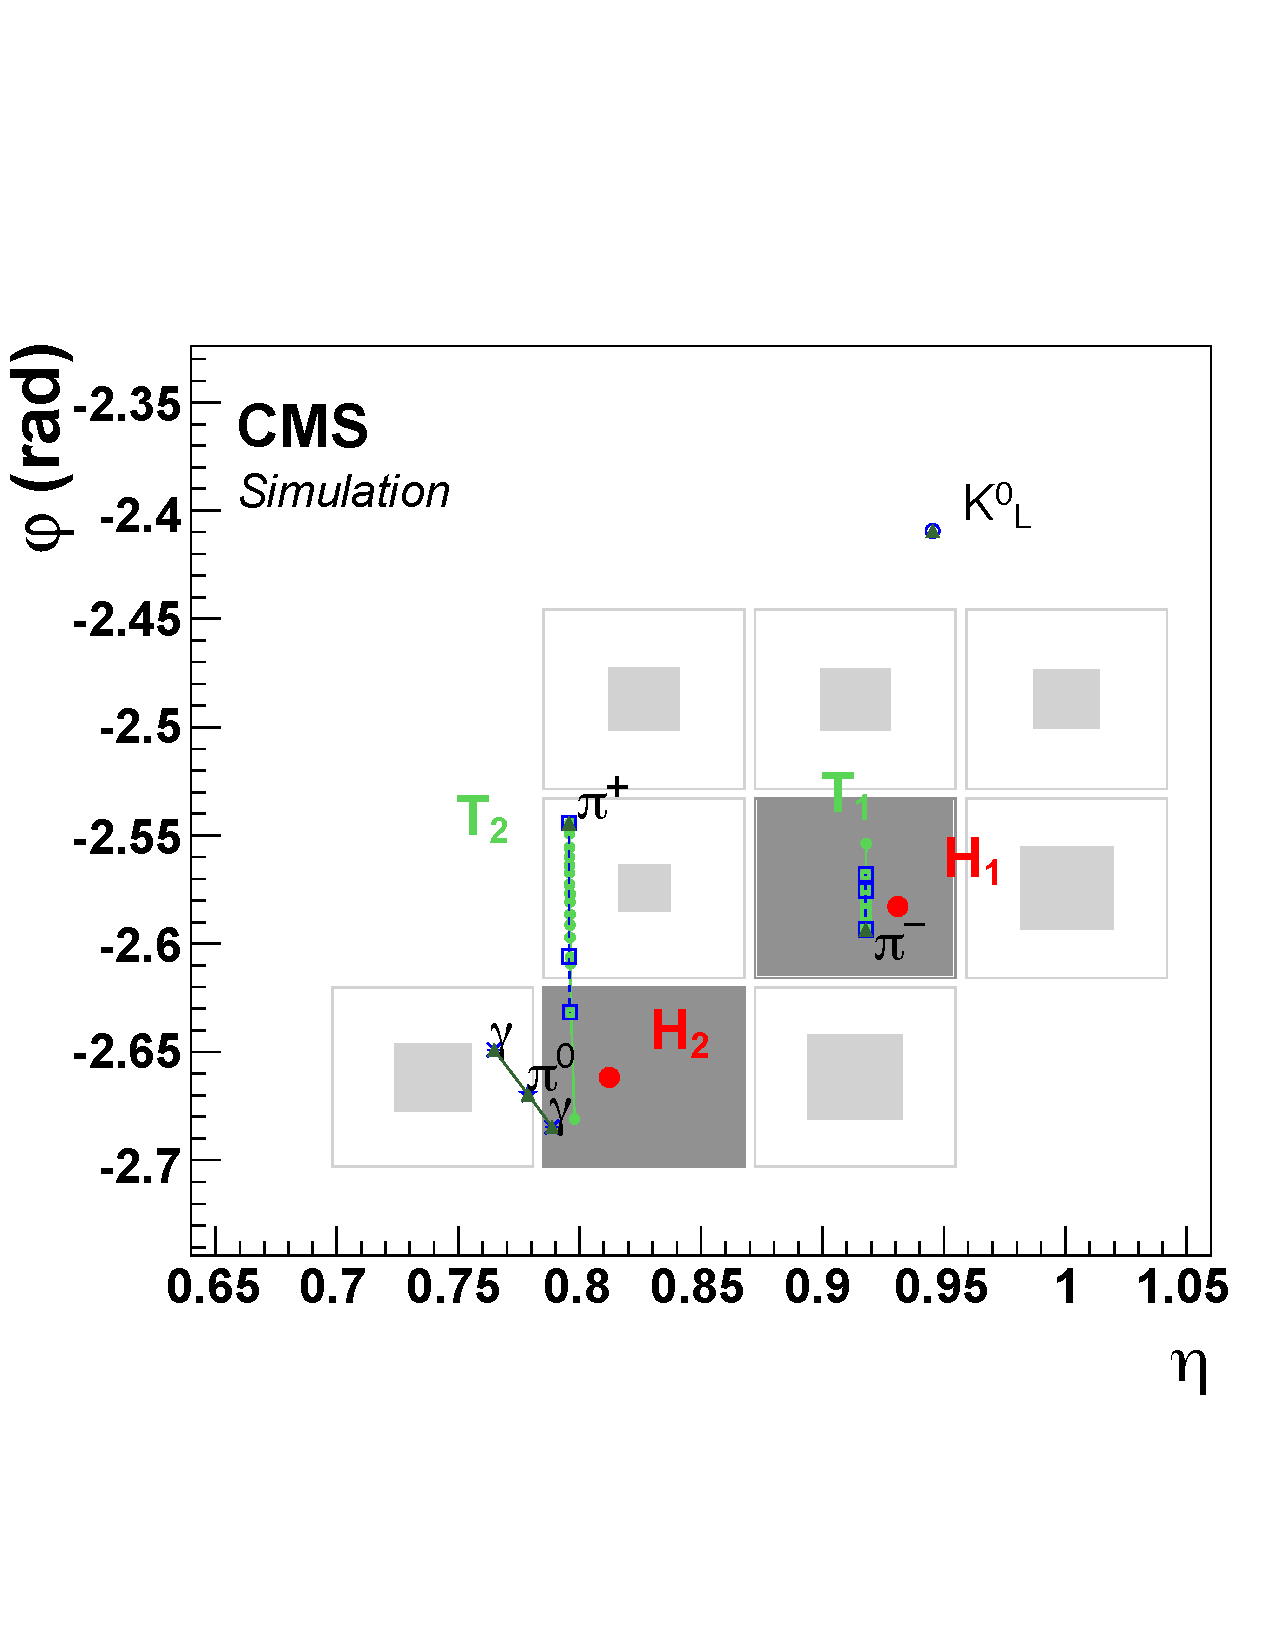
\includegraphics[scale=0.35]{images/hcalclusters}} \qquad
  }
  \caption[Event Display of Calorimeter Clusters]{An event display of a simulated jet of five particles projected onto A) the ECAL surface and B) the HCAL surface. The green lines represent reconstructed tracks while the red dots represent reconstructed cluster centroids. Four ECAL clusters and two HCAL clusters are shown.\cite{PARTICLEFLOW}}
    \label{fig:caloclusters}
\end{figure}

\subsubsection{Standalone muon tracks}\label{standalonemuontrack}

The muon chambers also reconstruct tracks from hits and, being the outer-most detector subsystems of the CMS detector, it is expected that these tracks represent muon trajectoriees. For drift tubes (DTs), hits are reconstructed along anode wires based on the measured arrival time of electrons produced when a traversing muon ionizes the gas in the drift cell. For cathode strip chambers (CSCs), hits are reconstructed from the intersection of clustered signals from cathode strips and anode wire groups. For resistive plate chambers (RPCs), the hits are reconstructed as the centroid of the clustered strip signals. Because the CSCs and DTs have multiple layers, as opposed to the single layer design of the RPCs, their hits are also locally reconstructed as \textit{track segments}.

Groups of DT and CSC track segments from the innermost chambers are used as seeds to generate trajectory candidates. A Kalman filter\cite{MUONKF} is used to form track candidates by combining the seed with track segments and hits found in the outer layers. This process is also repeated in reverse, from the outer layers towards the track seed, and the resulting pair is combined into a single track candidate which is then extrapolated to the beam axis and refit with a vertex constraint. This optimal track candidate, based solely on the information obtained by the muon chambers, is what is referred to as a \textit{standalone muon track}.

\subsection{Particle Candidates}

The PF algorithm identifies and reconstructs candidate electrons, photons, muons, and charged and neutral hadrons using the elements contributed by the various detector subsystems. Although not an exhaustive list, these five basic particle types are sufficient for the further reconstruction of more complex objects such as jets or \lept\ leptons. As discussed in the following sections, the benefits of this holistic approach towards particle reconstruction are realized as more robust particle candidates and improved estimates of their properties.

\subsubsection{Electrons}

Electron candidates are formed from seed tracks and their associated ECAL clusters which are compatible with the trajectory extrapolated from the track. The emission of photons by electrons as they travel through the silicon tracker poses a difficulty for the tracking algorithm which relies on pattern recognition, so a Gaussian-sum filter (GSF)\cite{GSFTRACK} is used to recover hits for the seed track which may have been missed during the trajectory building step. The direction of the seed track is taken to be the direction of the electron candidate and a combination of the seed track momentum and corrected ECAL cluster energies are used to assign the energy of the electron candidate.

This method of electron reconstruction achieves a high identification efficiency for genuine electrons but also tends to misidentify charged hadrons as electrons. The electron identification can be improved by training boosted decision tree (BDT) classifiers to discriminate against fake electrons using fourteen electron candidate features.\cite{CMSELEPERF} Those candidates with classifier scores above an analysis-dependent threshold are identified as electrons. The electron reconstruction efficiency as measured with a data sample of proton-proton collisions collected at $\sqrt{s} = 8\ \TeV$ and corresponding to an integrated luminosity of 19.7 \invfb\ is shown in Figure \ref{fig:elerecoeff}. The reconstruction efficiency is at least 85\% for electrons with $\pT > 15\ \GeV$ and plateaus at approximately 97\% for electrons with $\pT > 30\ \GeV$.

\begin{figure}[htbp]
  \centering
  \mbox{
    \subfigure [] {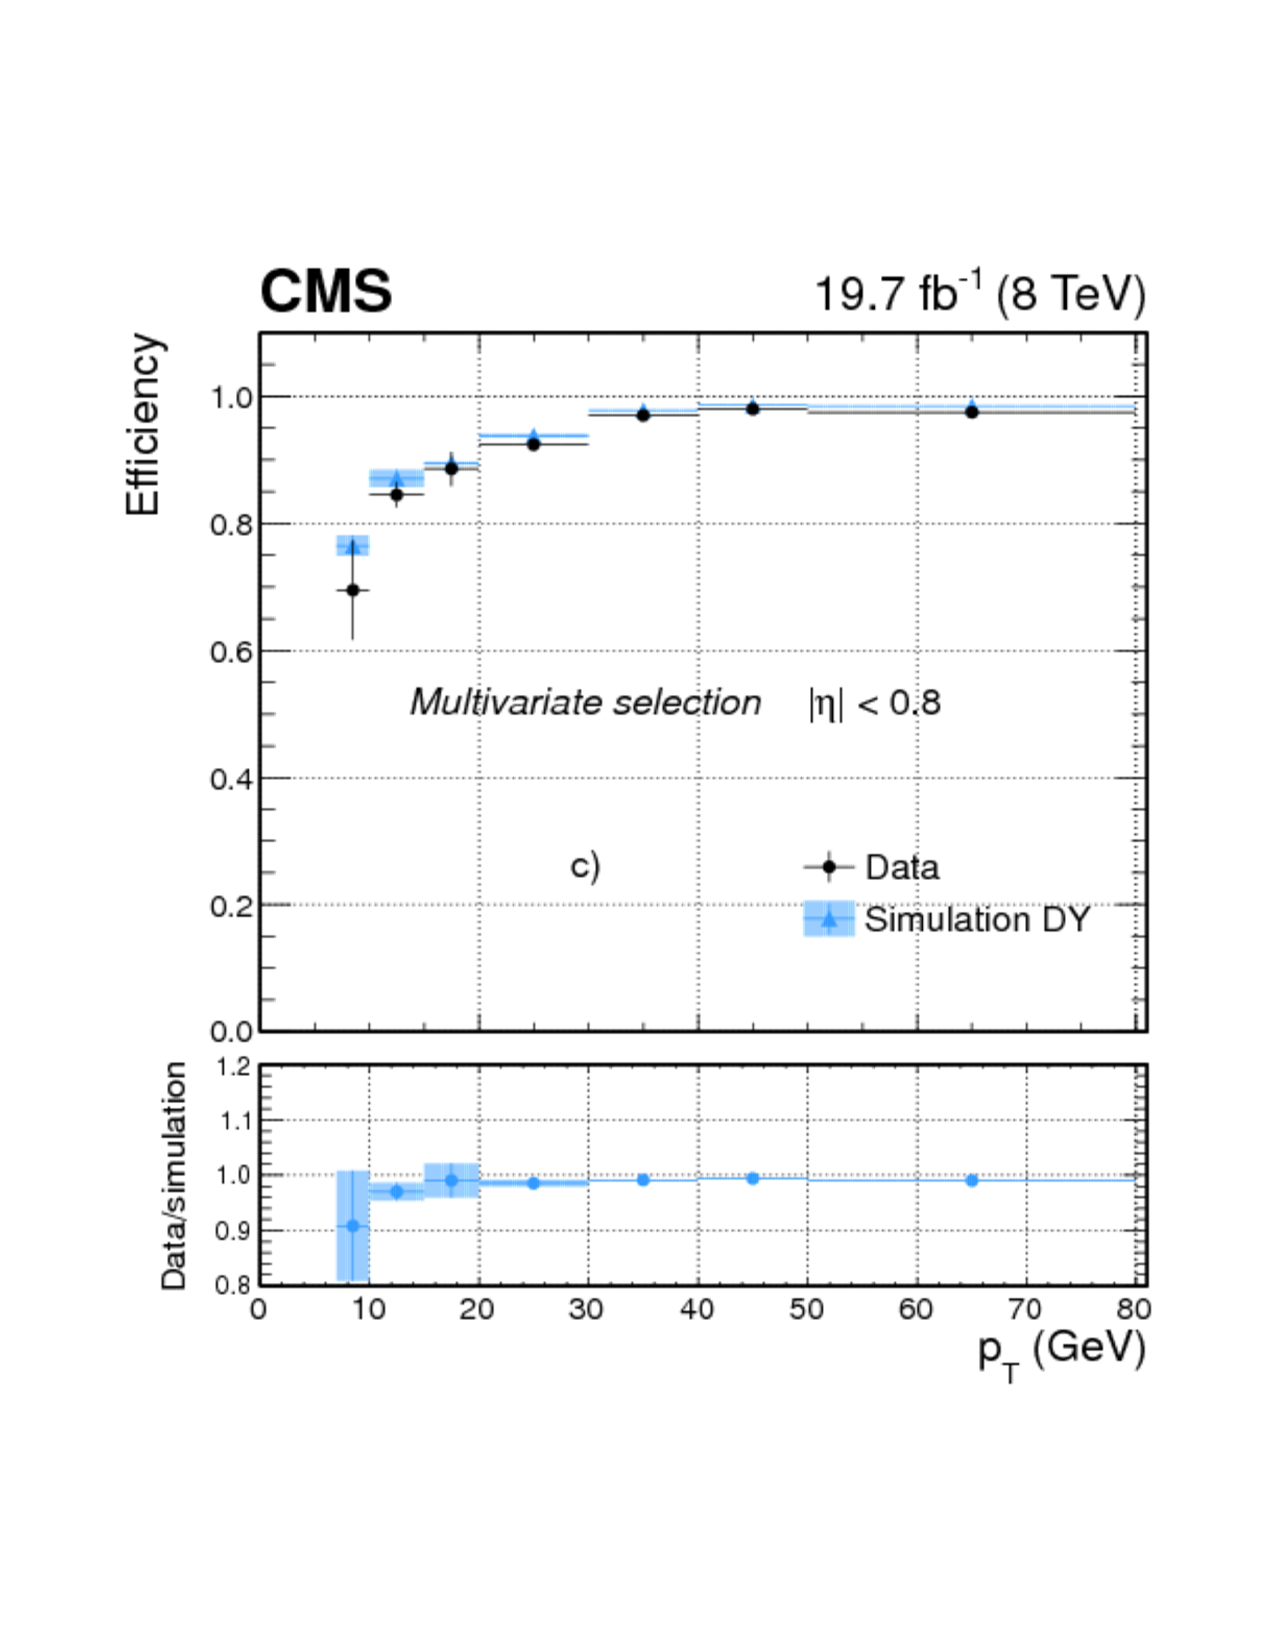
\includegraphics[scale=0.4]{images/elerecoeff_loweta}} \qquad
    \subfigure [] {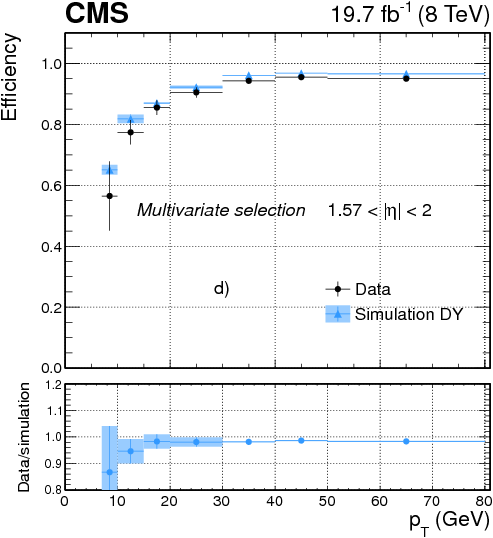
\includegraphics[scale=0.4]{images/elerecoeff_higheta}} \qquad
  }
  \caption[Electron Reconstruction Efficiency]{The electron reconstruction efficiency as a function of electron \pT\ for dielectron data events (black points) and Drell-Yan simulation (blue triangles) in regions of A) low $\eta$ and B) high $\eta$. The medium working point derived from the BDT classifier was used as the multivariate selection.\cite{CMSELEPERF}}
    \label{fig:elerecoeff}
\end{figure}

\subsubsection{Photons}

Photon candidates are seeded by ECAL superclusters which are not linked to a track. However, photons travelling through the silicon tracker are likely to interact with the material and convert into $e^{+}e^{-}$ pairs. To ensure that \textit{converted} photons are correctly reconstructed, pairs of oppositely-charged tracks identified as electrons are associated with the supercluster.

The identification of photons is also improved by training a BDT to discriminate prompt photons from background using features which describe the shape of the shower in the ECAL and aspects of the photon candidates supercluster.\cite{CMSPHOTPERF} Those candidates with classifier scores above an analysis-dependent threshold are identified as photons. The photon reconstruction efficiency measured with a data sample of proton-proton collisions collected at $\sqrt{s} = 8\ \TeV$ and corresponding to an integrated luminosity of 19.7 \invfb\ is shown in Figure \ref{fig:photrecoeff}. For the BDT threshold that achieves 80\% signal efficiency and approximately 93\% background rejection, the photon reconstruction efficiency typically falls between 80-90\% for photons with $\pT > 20\ \GeV$.

\begin{figure}[htbp]
  \centering
  \mbox{
    \subfigure [] {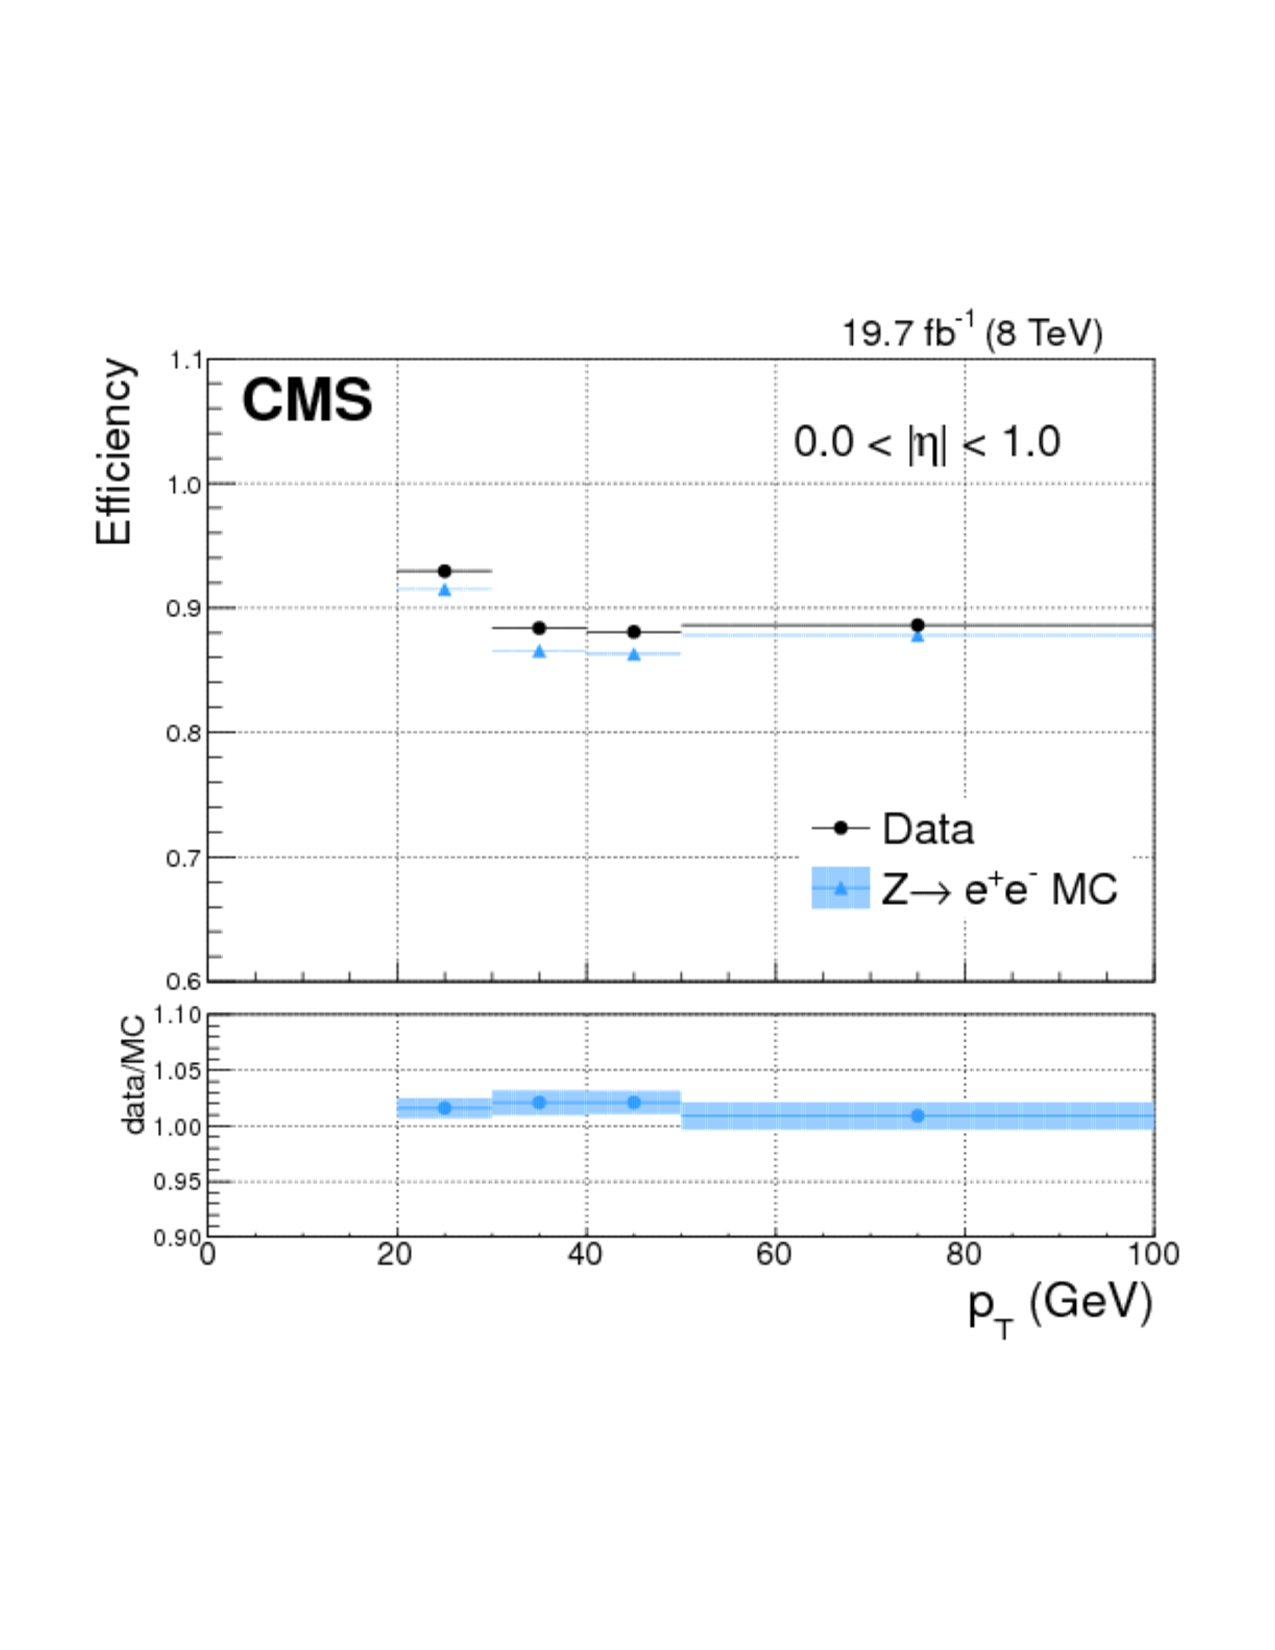
\includegraphics[scale=0.4]{images/photrecoeff_loweta}} \qquad
    \subfigure [] {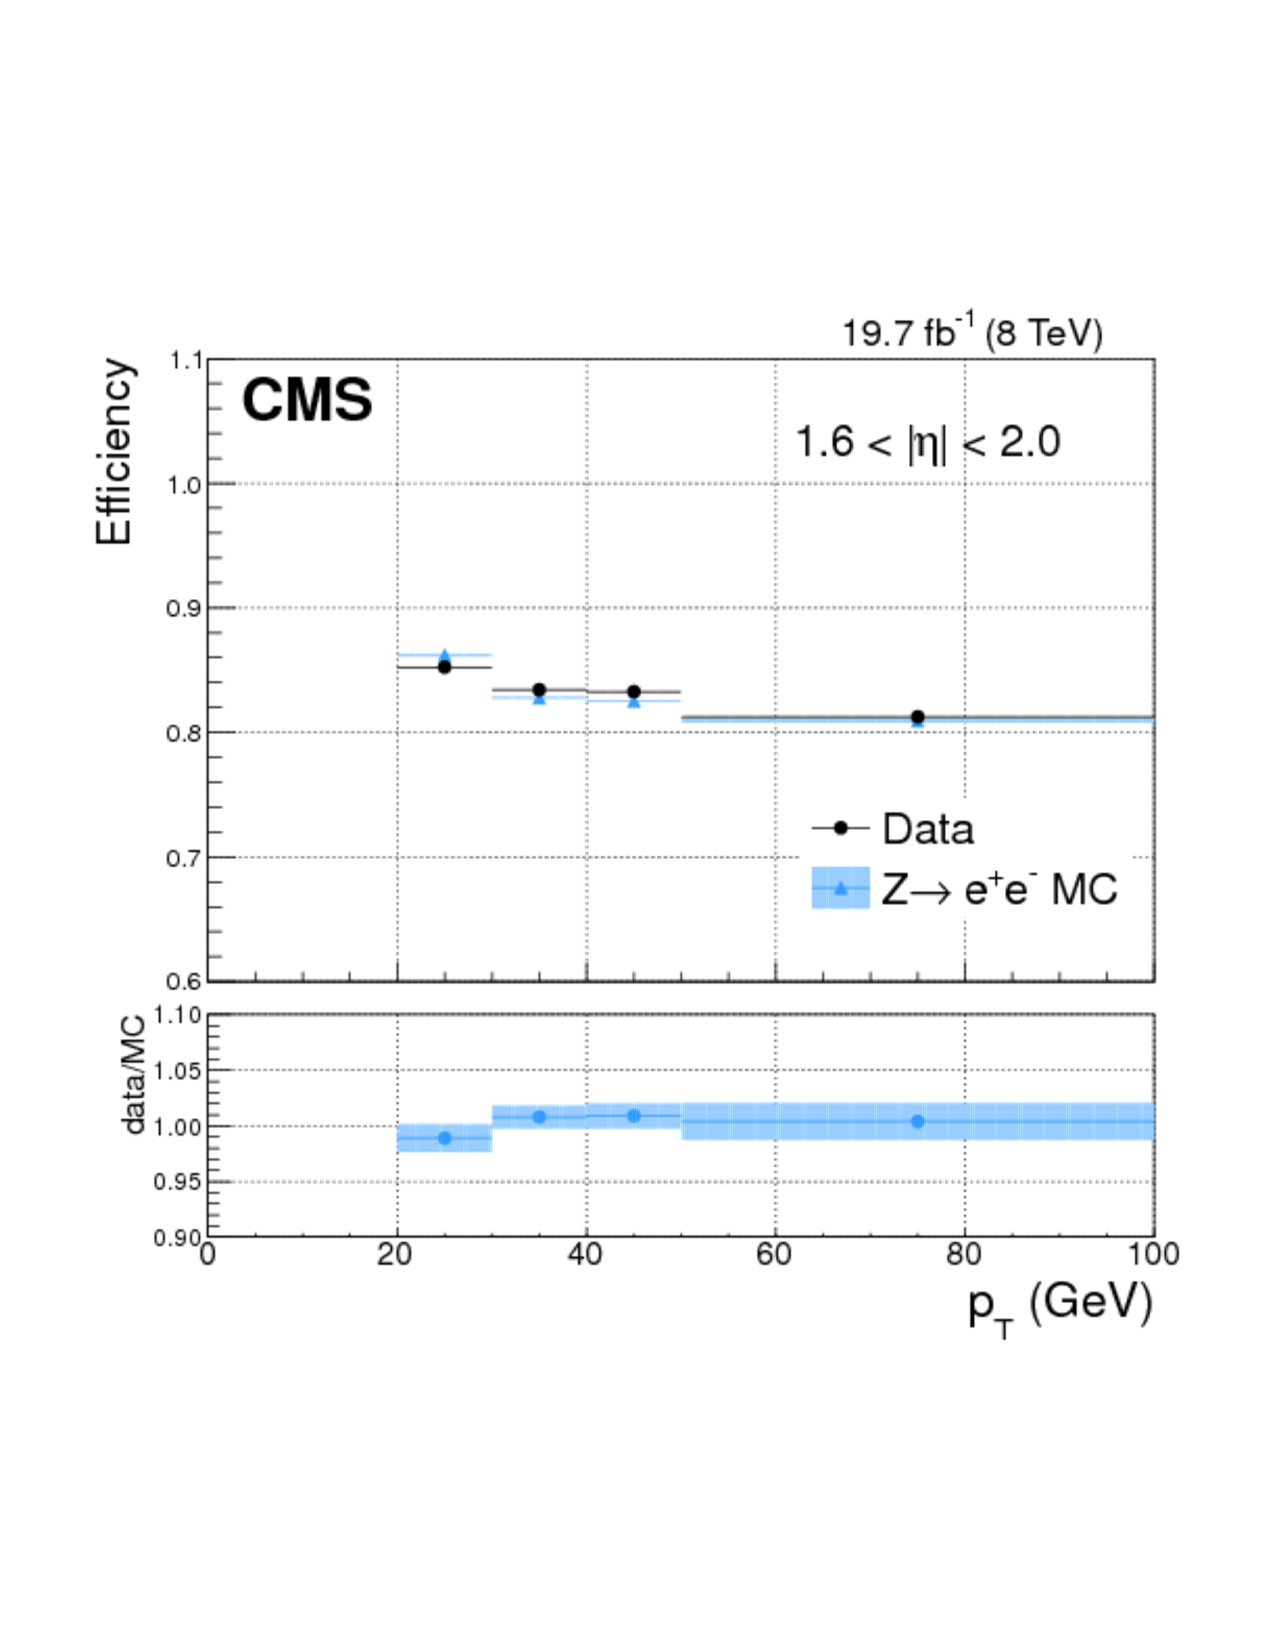
\includegraphics[scale=0.4]{images/photrecoeff_higheta}} \qquad
  }
  \caption[Photon Reconstruction Efficiency]{The photon reconstruction efficiency as a function of photon \pT\ for dielectron data events (black points) and Drell-Yan simulation (blue triangles) in regions of A) low $\eta$ and B) high $\eta$. An example working point for the BDT classifier which achives 80\% signal efficiency was used as the multivariate selection.\cite{CMSPHOTPERF}}
    \label{fig:photrecoeff}
\end{figure}

\subsubsection{Muons}

Muon candidates are seeded by standalone muon tracks, as well as \textit{tracker muon tracks} and \textit{global muon tracks} which are formed by combining information from the silicon tracker and muon chambers during the last two iterations of the iterative tracking algorithm. The tracker muon tracks are generated by an ``inside-out'' algorithm which extrapolates tracks from the silicon tracker which pass a momentum threshold to track segments identified in the DT and CSC chambers which are compatible with the hypothesized trajectory. Global muon tracks are similarly generated using an ``outside-in'' algorithm which extrapolates standalone muon tracks to tracks from the silicon tracker, followed by a combined Kalman filter fit. Those tracker muon tracks and global muon tracks which share silicon tracker tracks are identified as the same muon candidate. If any calorimeter clusters are associated with the muon tracks, they must be compatible with the energy deposition signature of a minimum ionizing particle.

A variety of muon identification algorithms are defined by the CMS Muon POG to serve the needs of different physics analyses. These algorithms combine low-level variables, such as the number of hits per track, and high-level variables, such as the compatibility between the tracks, track segments, and primary vertex, to identify specific types of muons under different conditions. For example, the common \textit{loose muon ID} is designed to efficiently identify tracker muons or global muons as prompt muons which originate from the primary vertex or light and heavy flavor decays.\cite{CMSMUONPERF} The reconstruction efficiency when using the loose muon ID, which exceeds 99\% over the full $\eta$ range, is measured using a 2015 data sample of proton-proton collisions collected at $\sqrt{s} = 13\ \TeV$ that corresponds to an integrated luminosity of approximately 2 \invfb\ and is shown in Figure \ref{fig:muonrecoperf}.

\begin{figure}[htbp]
  \centering
    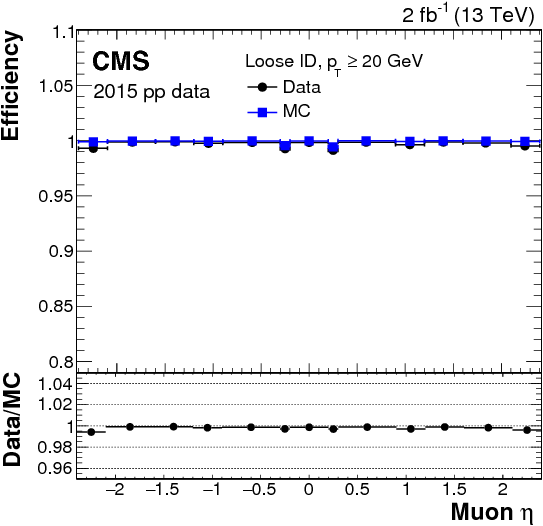
\includegraphics[width=3in]{images/muonrecoeff}
    \caption[Muon Reconstruction Efficiency]{The muon reconstruction efficiency as a function of $\eta$ for 2015 data events with a pair of reconstructed muons (black points) and Drell-Yan simulation (blue squares). The muon candidates were required to have $\pT > 20\ \GeV$ and pass the loose muon ID.\cite{CMSMUONPERF}}
    \label{fig:muonrecoperf}
\end{figure}

\subsubsection{Charged and neutral hadrons}

Charged hadron candidates are seeded by HCAL clusters which are linked to at least one track and possibly ECAL clusters. Neutral hadron candidates within the tracker's acceptance, or $\left| \eta \right| < 2.5$, are instead seeded by HCAL clusters which are not linked to a track while candidates utside of the tracker's acceptance are seeded by linked ECAL and HCAL clusters which present an energy excesses inconsistent with the signature of a charged hadron's energy deposition. Because such hadrons are created by the hadronization of final state particles, their performance is better discussed in the context of jet reconstruction and is reserved for section \ref{jetreco}.

\section{Primary Vertices}

Although multiple proton-proton interactions occur when the beams collide, only those interactions which cause the event to trigger are of interest. The position where such an interaction occurs is known as a \textit{primary vertex} and its reconstruction is vital because it the point of origin of the particles initially produced by the hard-scattering process.

The reconstruction of primary vertices begins with the clustering of tracks using a deterministic annealing algorithm.\cite{ITERTRACK} The tracks of each primary vertex candidate are then passed to an adaptive vertex fit to improve the estimate of the spatial position of the vertex.\cite{VERTEXFIT} The fit also assigns weights to each track in the cluster based on their compatibility with the primary vertex position, the sum of which is proportional to the number of degrees of freedom of the fit. Based on their fit results, only those candidates which have a $z$ position within 24 cm of the nominal detector center, a radial distance within 2 cm of the beamspot axis, and a vertex fit exceeding four degrees of freedom are considered primary vertices.

\section{Tau Leptons}

Besides the electron and muon candidates proposed by the PF algorithm, a third lepton remains to be reconstructed: the tau lepton. With a mass of $m_{\lept} \approx 1.78\ \GeV$\cite{PDG2018}, the tau is the only lepton able to decay hadronically through weak interactions, which accounts for almost two-thirds of its decays. The remaining decay channels are purely leptonic, with the tau decaying into either an electron of muon. The hadrons-plus-strips (HPS) algorithm\cite{TAURECO1,TAURECO2} is used to reconstruct the hadronically decaying taus by analyzing the constituents within reconstructed jets. The photons and electrons within the seed jets are clustered together into \textit{strips} because neutral pions, being the most common hadron produced by tau decays, predominantly decay into photon pairs. Based on the number of strips and charged particles found within the jet, a tau candidate is assigned to one of three possible decay topologies:
\begin{itemize}
  \item \textbf{One prong:} a single charged hadron and no strips.
  \item \textbf{Two prong:} a single charged hadron and one strip.
  \item \textbf{Three prong:} a single charged hadron and two strips, or three charged hadrons.
\end{itemize}
Finally, to reduce the misidentification rate of jets as taus, a BDT is trained to classify taus using jet features, such as the impact parameter of the leading track and the flight distance, as well as jet constituent features, such as the multiplicity of electrons and photons within the jet.

\section{Lepton Isolation}

Electrons and muons can either be prompt, produced directly by electroweak decays of massive particles suchs as the \bosW\ or \bosZ\ bosons, or non-prompt, produced by the subsequent decays of taus or jets. Lepton \textit{isolation}, a measure of the lack of activity around the charged particle track, is used to reconstruct prompt electrons and muons while rejecting leptons which are jet constituents. The isolation is defined as the ratio of the total transverse momentum of the particles within a cone around the lepton to the transverse momentum of the lepton itself
\begin{equation}
  I_{\mathrm{PF}} = \frac{1}{\pT} \left( \sum_{\bosg}\pT^{\bosg} + \sum_{h^{\pm}}\pT^{h^{\pm}} + \sum_{h^{0}}\pT^{h^{0}} \right),
  \label{eq:iso}
\end{equation}
where the superscripts indicate photons (\bosg), charged hadrons ($h^{\pm}$), and neutral hadrons ($h^{0}$) and the lack of a superscript denotes the lepton of interest. The identification of prompt leptons proceeds by placing thresholds directly on the lepton isolation, with lower thresholds indicating a tighter criterion, or passing the lepton isolation as one of several inputs to a classifier.

\section{Jets}\label{jetreco}

The experimental signature of quarks and gluons produced by a hard scattering process are collimated sprays of particles known as \textit{jets}. Due to color confinement, quarks and gluons are not observed directly but through the hadrons they immediately form, which are themselves unstable and inferred from the decay of their partons. This process of hadronization and fragmentation continues until the hadrons are absorbed or the remaining decay products are stable particles. Because jet constituents leave signatures all throughout the detector volume, the holistic approach of the PF algorithm is well-suited for jet reconstruction.

\subsection{Reconstruction}

The primary concerns for jet reconstruction are the identification and association of a jet's constituent particles. The identification of possible constituent particles is undertaken by the PF algorithm, where prompt and isolated electrons, muons, and photons are removed from consideration. The assocation of constituents to form a jet is handled by specialized jet finding algorithms.

Jet finding algorithms broadly fall under two categories, cone algorithms and sequential recombination algorithms. Cone algorithms use a ``top-down'' approach based on the assumption that jets can be contained within conical envelopea. Cones of radius $R$ are first seeded along regions of energy flow and stable cones, which have axes compatible with the direction of the vectorial sum of the momenta of particles within the cone, are kept. Overlapping stable cones are further split or merged under the algorithm converges. Sequential recombination algorithms instead use a ``bottom-up'' approach based on the assumption that jet constituents form well-defined clusters due to their collimation. Distance metrics in coordinate space and in transverse momentum space are defined and calculated between pairs of constituent candidates, with the minimum distance pair of either space used to seed the jet cluster. The distances are then recalculated and candidate particles combined with the jet cluster iteratively until reaching a stop condition.

Because the theoretically motivated observable quantities describing parton decays are manifested experimentally as the properties of reconstructed jets, the implementation of jet finding algorithms must be infrared and collinear (IRC) safe. Jet finding algorithms are IRC unsafe if they are sensitive to soft emissions, such as gluon radiation, and collinear splittings of particles as illustrated in Figure \ref{fig:IRCunsafe}. By satisying the requirement of IRC safety, the jets reconstructed by the algorithm may be considered valid approximations of the final state partons.

\begin{figure}[htbp]
  \centering
  \mbox{
    \subfigure [] {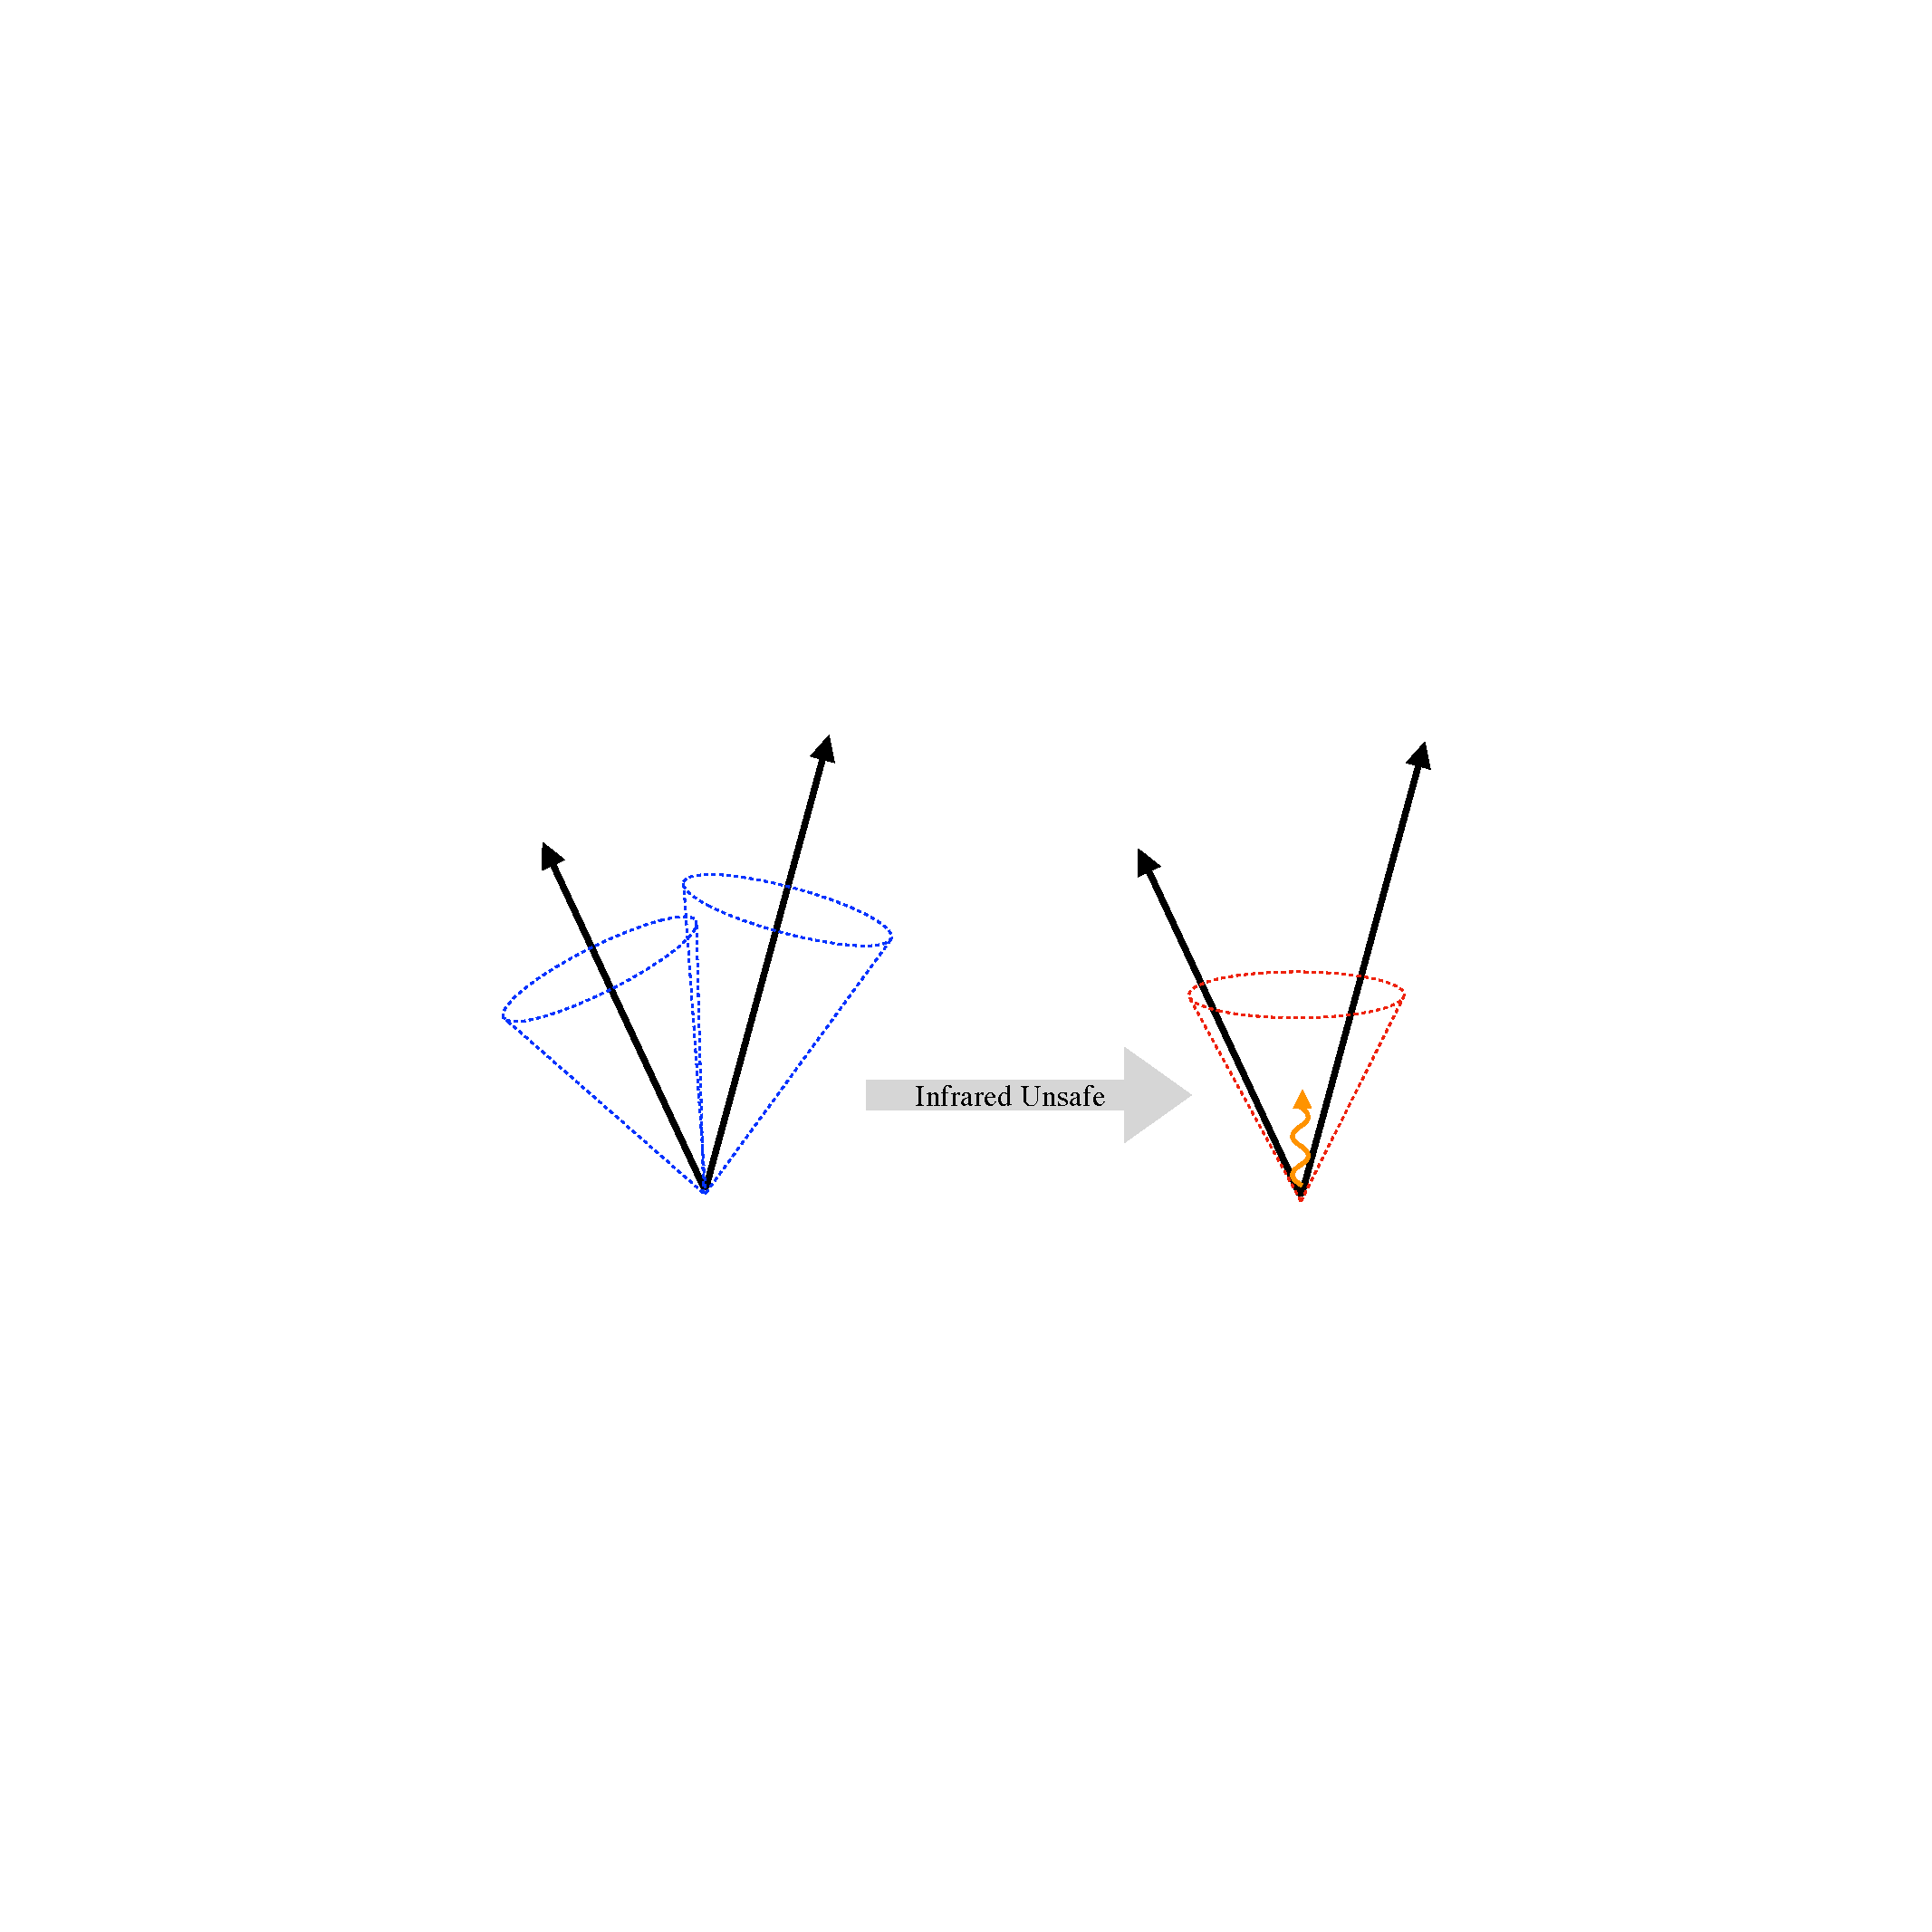
\includegraphics[width=3in]{images/infrared_emission}} \qquad
    \subfigure [] {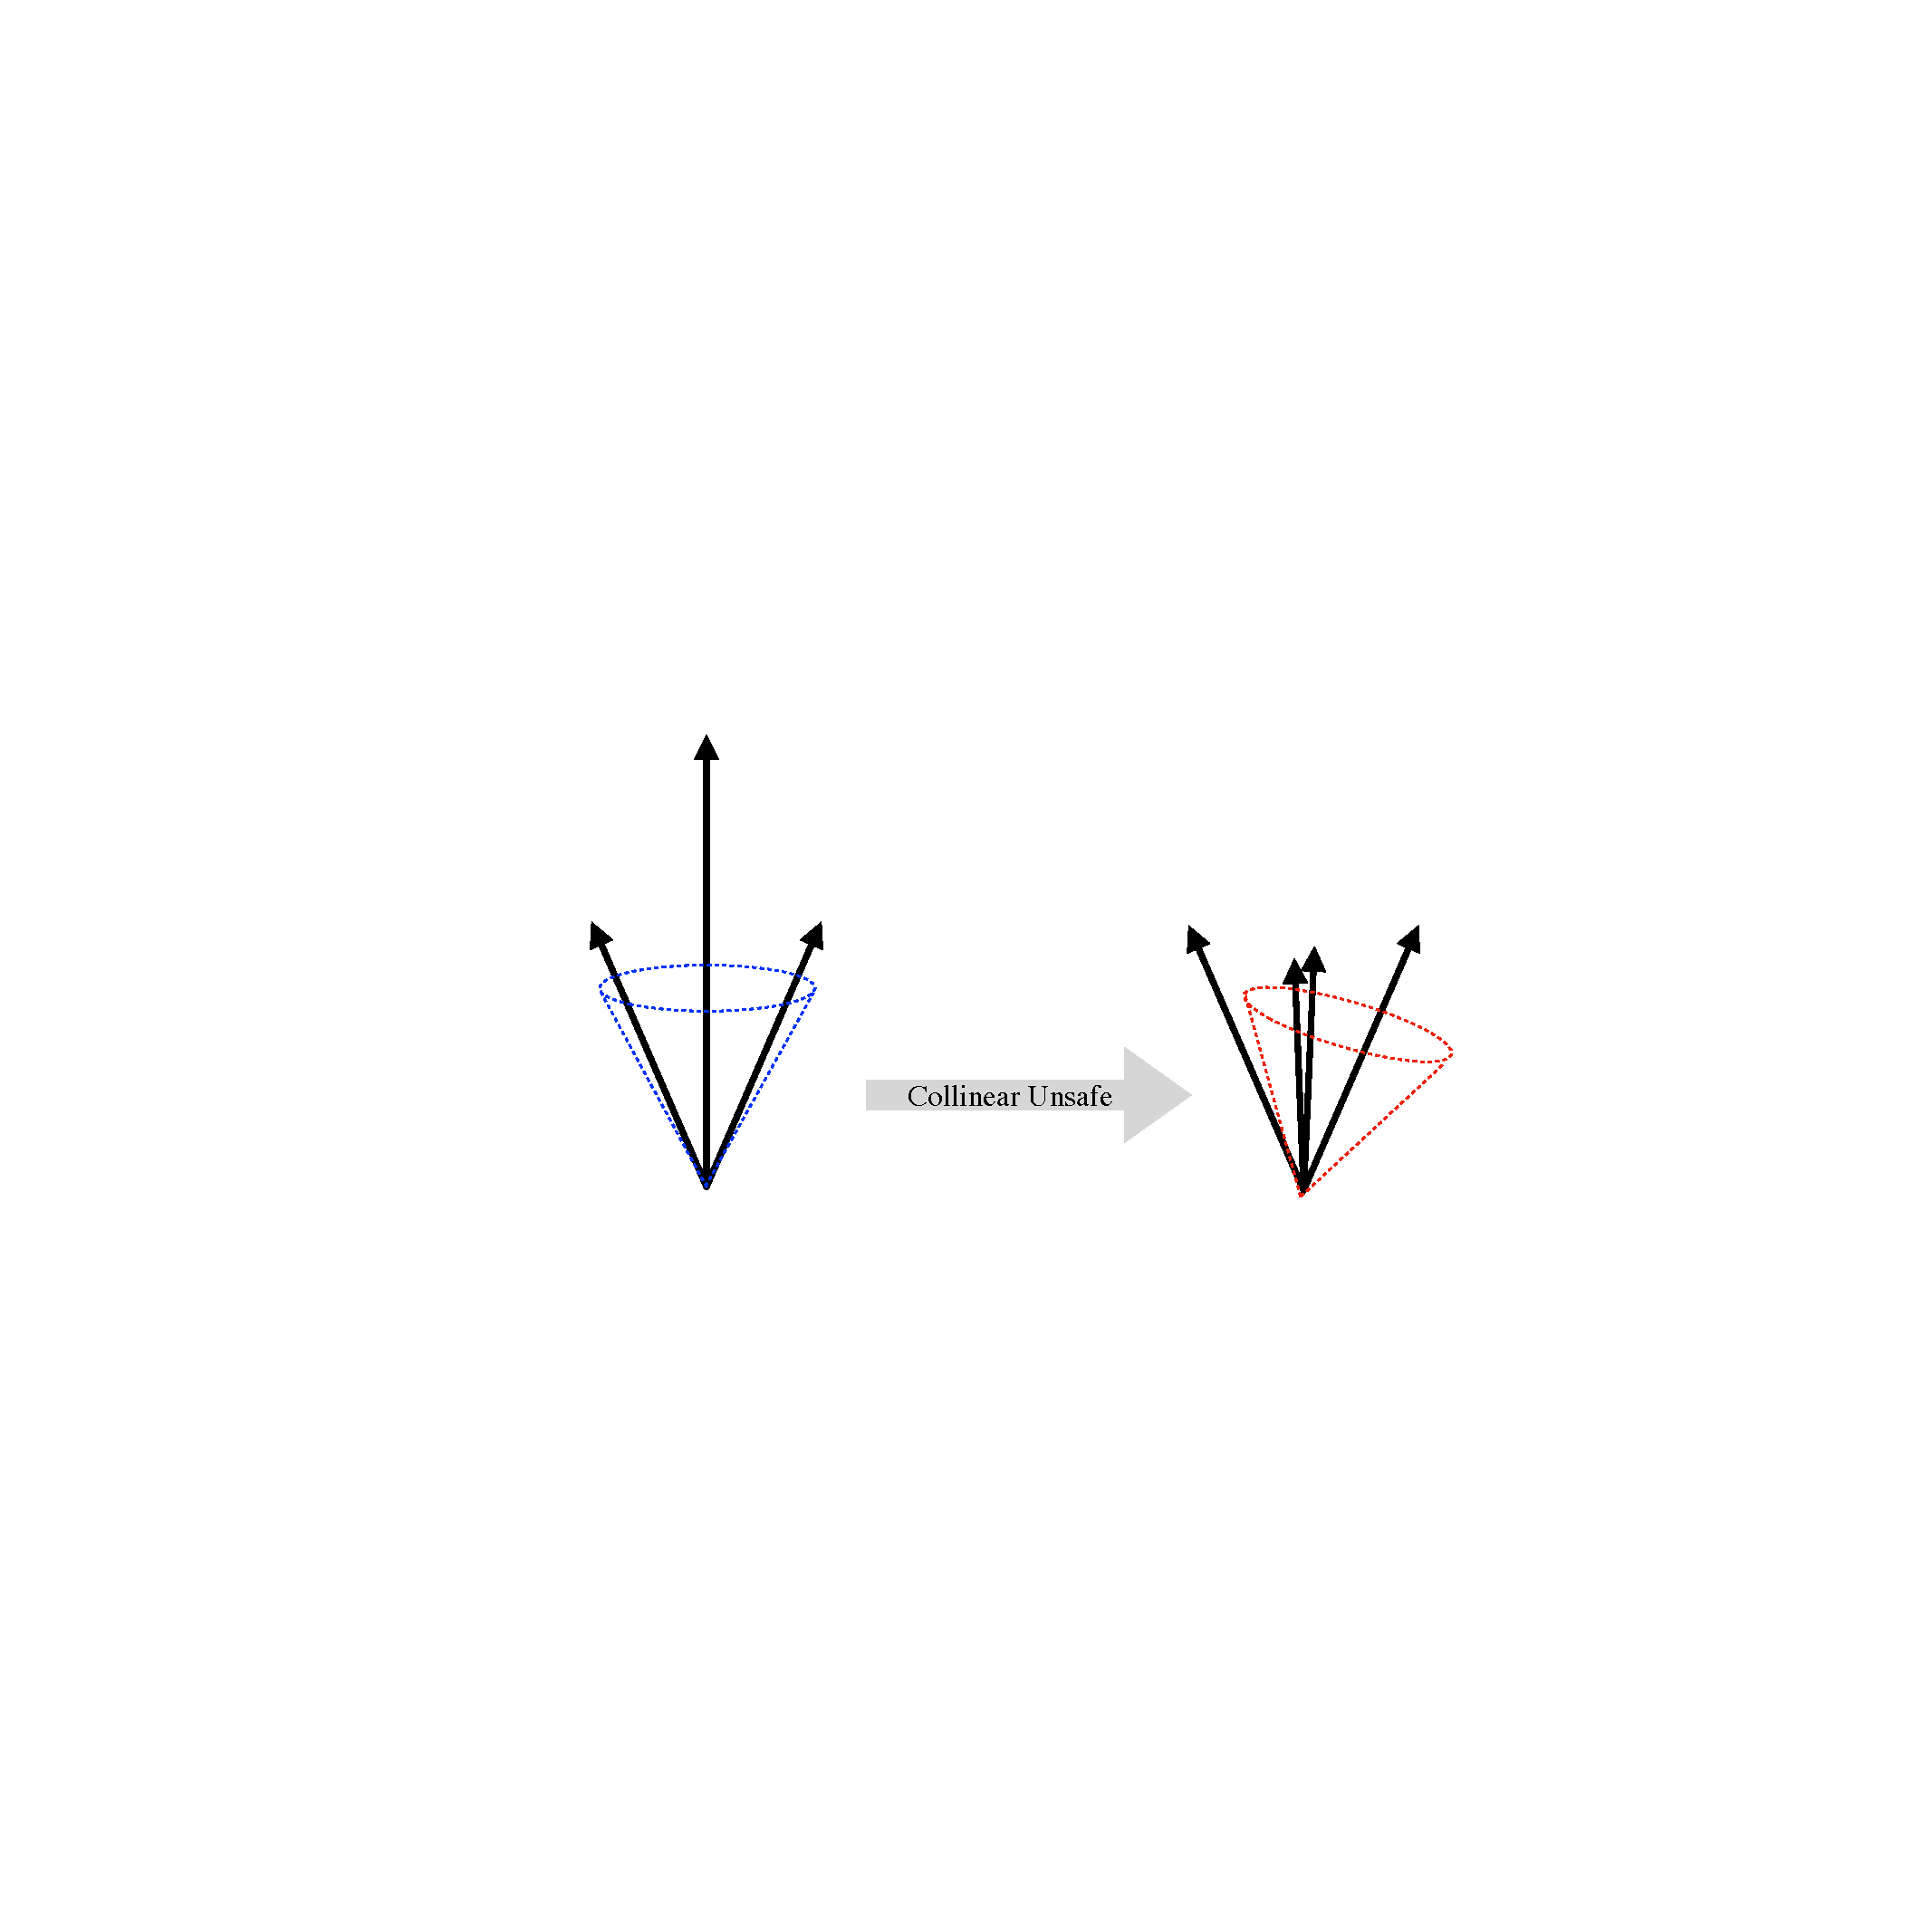
\includegraphics[width=3in]{images/collinear_emission}} \qquad
  }
  \caption[Infrared and Collinear Unsafety]{An illustration of the consequences of infrared and collinear unsafety for jet finding: A) an example of infrared unsafety, where a soft emission (orange) causes the algorithm to merge two overlapping but otherwise distinct jets; B) an example of collinear unsafety, where the collinear splitting of a contituent alters the jet returned by the algorithm.}
    \label{fig:IRCunsafe}
\end{figure}

Although cone algorithms were previously favored for their ease of implementation, simple jet geometries, and faster execution compared to sequential recombination algorithms, the vast majority of cone algorithms are not IRC safe. With the release of the \texttt{FastJet}\cite{FASTJET} software package, efficient implementations of sequential recombination algorithms with $\mathcal{O}(n \log n)$ time complexity were readily adopted at the LHC. The CMS experiment uses the \textit{anti-$k_{T}$} jet clustering algorithm\cite{ANTIKT} to reconstruct jets from PF candidates. The anti-$k_{T}$ algorithm defines the distance in transverse momentum space as
\begin{equation}
  d_{ij} = \min \left( \frac{1}{p_{Ti}^{2}}, \frac{1}{p_{Tj}^{2}} \right) \times \frac{R_{ij}^{2}}{R},
  \label{eq:antikt_dij}
\end{equation}
where $i$ and $j$ are the indices of the PF candidates, $R$ is the radius parameter which governs the size of the reconstructed jets, and $R_{ij}^{2}$ is the Euclidean distance between the PF candidates in the $\eta\phi$-plane
\begin{equation}
  R_{ij}^{2} = \left( \eta_{i} - \eta_{j} \right)^{2} + \left( \phi_{i} - \phi_{j} \right)^{2}.
  \label{eq:deltaR2}
\end{equation}
The anti-$k_{T}$ algorithm also defines an additional distance between the beam axis and the $i$-th particle to be
\begin{equation}
  d_{iB} = \frac{1}{p_{Ti}^{2}},
  \label{eq:antikt_diB}
\end{equation}
which is used to classify a finished cluster as a jet.

The algorithm proceeds by finding the minimum over the set of distances $\left\{ d_{ij}, d_{iB} \right\}$. If the minimum distance is between a pair of particles $i$ and $j$, their four-vectors are summed to form a new particle and particles $i$ and $j$ are removed from the set of particles consideredby the algorithm. If the minimum distance is between a particle and the beam axis, the particle is considered a jet and removed from the set o particles considered by the algorithm. The algorithm continues until all initial particles have been combined into jets. Because the distance measure given by Equation \ref{eq:antikt_dij} is dominated by high \pT\, the anti-$k_{T}$ algorithm tends to cluster soft particles with the hardest particles first,producing perfectly conical jets.

\subsection{Energy Scale and Resolution Corrections} \label{jesjer}

Disagreements between the measured energies of reconstructed jets and the true energies of their corresponding partons are expected. The jet's constituent particles encounter unavoidable energy losses as they travel through the detector material and their measured energies are biased by the non-linear response of the detector subsystems to their signals. Because the four-momentum of a jet is taken to be the vectorial sum of the momenta of its clustered PF candidates, these issues and more are compounded together and require a dedicated calibration.

In order to calibrate jet energies, the recommended procedure by the CMS experiment applies a series of \textit{jet energy scale} (JES) corrections which scale the four-momentum of jets. The various detector effects are addressed using a factorized approach shown in Figure \ref{fig:jeschain}, where each of the corrections are designed to target specfic effects and are applied in a fixed-order sequence.

\begin{figure}[htbp]
  \centering
    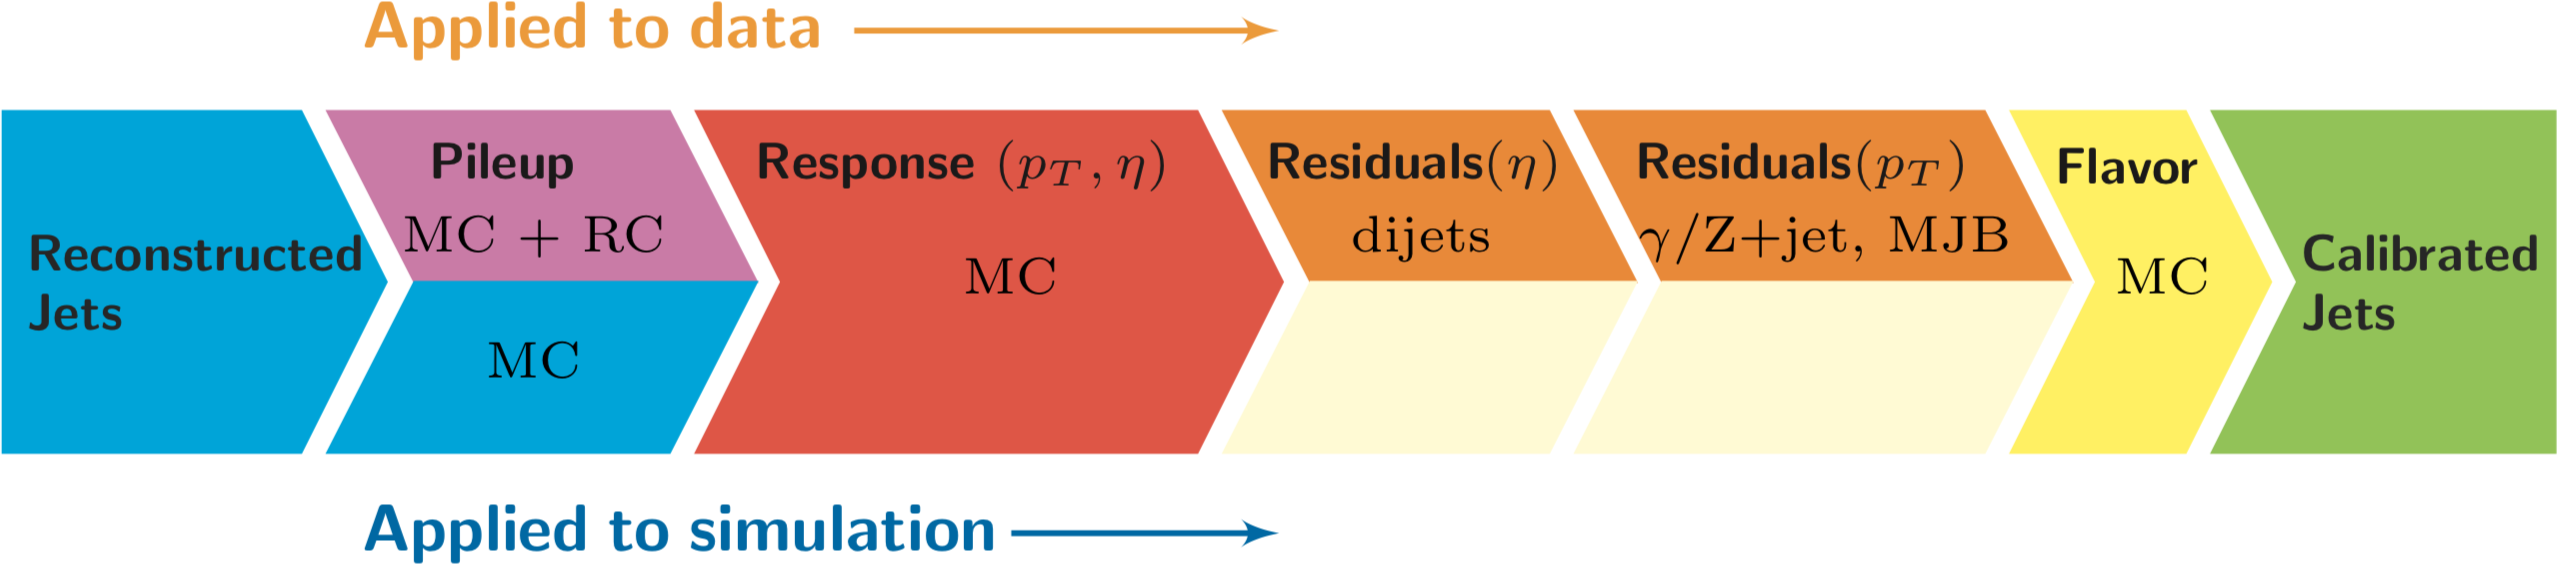
\includegraphics[width=6in]{images/jeschain}
    \caption[Jet Energy Scale Corrections Infographic]{An inforgraphic of the jet energy scale corrections used by the CMS experiment for data and Monte-Carlo (MC) simulated samples. Corrections derived from simulation are marked with MC, while RC stands for random cone and MJB stands for multijet background.\cite{CMSJES}}
    \label{fig:jeschain}
\end{figure}

\subsection{\qrkb-Tagging}

\section{Missing Transverse Energy}

\subsection{Corrections}

\subsection{Filters}

